 %!TeX root = ../main.tex
\chapter{非热化电子动理学数值研究}
\section*{引言}
电子回旋辐射强度变化追根溯源上是电子速度分布改变。为了理解放电实验过程中电子回旋辐射特征,必先理解非热化电子速度分布的演化,而分布的演化需要考虑电场、磁场、电磁波与等离子体相互作用。根据第二章的介绍,动理学过程是由一组非线性偏微分方程描述,目前还没有准确的解析解来表示速度分布函数随时间的变化,因此数值分析成为求解动理学演化过程中必要的手段。


动理学是描述等离子体的根本方法,在研究等离子体中的地位就如同流体力学在空气动力学中的地位。动理学数值研究平台使我们能够站在前人的理论基础上研究放电过程中非热化电子演化,能够在不同的外界参数下对等离子体分布函数的演化行为做出预测。这就像是流体力学数值平台,流体力学数值研究平台使得预测天气,优化飞机气动结构以及任何与流体有关的工程设计成为可能。而掌握了等离子体动理学方程的数值平台,就具备了优化托卡马克放电,以及预测各种放电条件下等离子体的演化等能力。描述等离子体电子离子的相互作用的另一种方法是基于第一
性原理PIC程序\cite{RN2071},但是PIC程序对计算资源、程序的性能要求非常高,很难模拟托卡马克放电过程中密度为$10^{19}/m^3$,时间为秒量级的物理过程尺度。而动理学方程从统计的角度出发,对特定物理问题具有更高效的计算速度,而且能够满足托卡马克部分放电条件下等离子体物理过程模拟,因此随着时间推移动理学数值平台必然在未来的核聚变研究中起到举足轻重的作用。
\par 动理学数值研究最早由加州理工学院H. B. Keller等一众科学家与20世纪60年代发起,他们的研究从均匀磁场位型到非均匀磁场位型,从磁镜装置到托卡马克装置,涉及面之广,内容之繁多为后人的研究提供了丰富的参考资料, J. Killeen在书《磁约束等离子体动理学计算方法》\cite{RN1827}对此有详细介绍。2014年麻省理工学院以Matt Landreman为代表的科学家利用谱方法开发了CODE程序用于逃逸电子同步辐射数值计算\cite{RN814};2017年查尔姆斯理工大学A. Stahl利用面向对象编程编写的NORSE程序\cite{RN1894}实现了对动理学非线性碰撞项数值求解,为研究主体等离子体动理学特征提供计算平台;2018年普林斯顿大学刘畅通过有限元方法数值求解动理学方程研究了等离子体哨声波不稳定性对分布函数的影响\cite{RN1815}。

本章动理学求解方法结合了CODE的谱方法和NORSE程序的面向对象编程思想实现了空间维度为0D2P(零个位置空间,两个动量空间)分布函数演化数值计算,其中包含了电场驱动项,试探粒子碰撞项、回旋辐射阻尼项、以及目前最完备的逃逸电子雪崩项等物理过程,可以根据放电过程中密度、环电压等时变背景参数研究动理学方程的动态演化过程。相对于过去的动理学计算程序,本论文的计算方法兼顾了计算效率,结合时下最完备的雪崩算符,利用面向对象编程技术可用于求解动态背景环境中非热化电子分布函数的演化过程。




本章主要介绍动理学数值平台的算法和测试,为了从第一性原理角度理解反常多普勒效应对电子运动的影响,在介绍等离子体和电磁波相互作用时首先从单电子和电磁波相互作用入手,通过数值的方法研究电子的动力学行为,然后进一步对波和等离子体相互作用展开探讨,研究了利用电磁波抑制逃逸电子方法的可能性。由于电磁湍动项过于复杂,限于时间和个人能力,目前的动理学系统并没有完成对电磁湍动项的数值求解,在今后的研究中将会进一步完善相关模块。
\section{均匀电磁场中动理学演化过程数值模拟}
模拟非热化电子回旋辐射需要准确的电子动量空间分布信息。对于逃逸电子,由于其速度分布函数远偏离麦克斯维分布并且无法用简单的双温模型准确描述,因此通过动理学方程求解非热化电子速度分布对计算电子回旋辐射尤为重要。这里考虑这样一种背景设定,等离子体处在均匀电场背景和磁场背景中,速度分布函数动量空间坐标为$(p,ξ)$,p表示约化动量,约化因子为$m_e c,ξ=p_∥/p$表示电子散射角的余弦。对于逃逸电子,影响动量空间分布的重要参数包括静电场、等离子体碰撞率、辐射阻尼、大角度雪崩效应以及电磁湍动过程。根据\autoref{sec:chapt2}的描述,该过程可表示为:
\begin{equation}
\frac{\partial f}{\partial t}-\mathrm{e} E_{\|}\left(\xi \frac{\partial f}{\partial p}+\frac{1-\xi^{2}}{p} \frac{\partial f}{\partial \xi}\right)+C[f]+\frac{\partial}{\partial \boldsymbol{p}} \cdot \boldsymbol{F}_{\mathrm{rad}} f+\widehat{L}[f]=\hat{S}_{A}[f]+\hat{S}_T[f]
\end{equation}
为了使每个过程清晰明了,本章首先介绍本文所基于的数值模拟方法,然后分别研究Fokker-Plank方程 $C[f]$,辐射阻尼效应$∂/∂p⋅F_{rad} f$,以及雪崩效应$S_A [f]$对分布函数演化的影响。
\subsection{基于谱方法的数值模拟}
通过选取适当的函数基将分布函数展开为谱函数形式,通过求解谱函数的系数演化方程来获得分布函数的演化的方法称为谱方法。相对于有限元和有限差分,在相同计算成本下谱方法由于其自身高精度和快速收敛等优势成为求解偏微分方程的主要手段之一\cite{RN2027}。首先使用谱方法对动理学方程数值求解是Matt Landreman\cite{RN814},Matt Landreman利用谱方法求解动理学在碰撞项作用下的演化并将其程序命名为CODE(COllisional Distribution of Electrons),而后2016年stahl\cite{RN1809}		结合CODE程序分析等离子体背景参数随时间演化下逃逸电子的动理学行为,2018年O. Embréus\cite{RN1811}	使用CODE程序分析了雪崩电子碰撞项对分布函数的影响,谱方法在求解动理学方程中已成为一种主流方法。本文采用的谱方法借鉴了CODE程序的思想,介绍如下:\par
首先对动理学方程无量纲化, 将方程两边同时乘以$\frac{m_{e}^{3} v_{e}^{3} \pi^{\frac{3}{2}}}{v_{c c} n} $, 其中 $ v_{e}=\sqrt{\frac{2 T}{m_{e}}}$ , $ v_{c c}=\frac{e^{4} n \ln \Lambda}{4 \pi \epsilon_{0}^{2} m_{e}^{2} c^{3}}$ , 并对动量 $ p_{m v}  $无量纲化为 $ p=\frac{p_{m v}}{m_{e} c} $, 归一化后的分布函数为$F=\frac{\pi^{\frac{3}{2}} m^{3} v_{e}^{3}}{n} f$, 当  p  趋向于 0时, $F \rightarrow 1$。$ \hat{E}=\frac{E}{E_{c}}$ , 其中  $E_{c}=\frac{m_{e} c v_{c c}}{e}  $为 Connor 电场, 只有电场$  |E|>   \left|E_{c}\right|$  才有可能出现逃逸电子\cite{RN1875},约化时间$ \hat{t}=v_{c c} t$ , 此时方程可表示为:
\begin{align}\label{eq:Specnorm}
\frac{\partial F}{\partial \hat{t}}+\widehat{\mathrm{E}}\left(\xi \frac{\partial F}{\partial p}+\frac{1-\xi^{2}}{p} \frac{\partial F}{\partial \xi}\right)+\hat{C}[F]+\frac{\partial}{\partial \boldsymbol{p}} \cdot \widehat{\boldsymbol{F}_{\mathrm{rad}}} F+\widehat{L}[F] & = \hat{S}_{A}[F]+\hat{S}_{T}[F]\end{align}
将F用Legendre 多项式$P_L (ξ)$展开:
\begin{equation}
F(p, \xi)=\sum_{n=0}^{\infty} F_{n}(p) P_{n}(\xi)
\end{equation}
然后将运算符
\begin{equation}
\frac{2 m+1}{2} \int_{-1}^{1} \mathrm{P}_{\mathrm{m}}(\xi)(\cdot) d \xi
\end{equation}
作用在动理学方程两边得到谱函数:
\begin{equation}\label{eq:Fnm}
\frac{\partial F_{m}}{\partial \hat{t}}+\sum_{n=0}^{\infty}\left\{\hat{E}_{n m}(F)+\hat{C}_{n m}(F)+\hat{R}_{n m}(F)+\hat{L}_{n m}[F]\right\}=\hat{S}_{A}[F]+\hat{S}_{T}[F]
\end{equation}
其中
\begin{equation}
\frac{2 m+1}{2} \int_{-1}^{1} \mathrm{P}_{\mathrm{m}}(\xi)\cdot P_n(\xi) d \xi=\left\{\begin{alignedat}{2}
&1,& \qquad m=n \\
&0,& \qquad m\neq n 
    \end{alignedat}
  \right.
\end{equation}
下面对每一项分别展开介绍
\begin{enumerate}
\item
电场驱动项为
\begin{equation}
\hat{E}_{n m}(F)=\hat{E} \frac{\partial F_{n}}{\partial p} Q_{n m}+\frac{\hat{E} F_{n}}{p} U_{n m}
\end{equation}
其中
\begin{align}Q_{n m} & = \frac{2 m+1}{2} \int_{-1}^{1} \xi \mathrm{P}_{\mathrm{m}}(\xi) \mathrm{P}_{\mathrm{n}}(\xi) d \xi\\ \quad U_{n m} & = \frac{2 m+1}{2} \int_{-1}^{1}\left(1-\xi^{2}\right) \mathrm{P}_{\mathrm{m}}(\xi) \frac{d \mathrm{P}_{\mathrm{n}}(\xi)}{d \xi} d \xi\end{align}
\item
碰撞项\cite{RN2025}:
\begin{equation}
\left.\hat{C}[F] = \left(v_{\mathrm{D}}^{\mathrm{ee}}+v_{\mathrm{D}}^{\mathrm{ei}}\right) \mathcal{L}\{F\}+\frac{1}{p^{2}} \frac{\partial}{\partial p}\left[p^{3}\left(v_{\mathrm{S}}^{\mathrm{ee}} \mathrm{F}+\frac{1}{2} v_{\|}^{\mathrm{ee}} p \frac{\partial \mathrm{F}}{\partial p}\right)\right]\right]
\end{equation}
如\autoref{eq:tpfok}所述,其中碰撞频率$\nu_D^{ee}$、$\nu_D^{ei}$ 表征电子-背景电子、电子-背景离子碰撞过程中速度方向散射
速率,$\nu_S^{ee}$描述了电子与背景电子碰撞而减速的速率,$\nu_{∥}^{ee}$表示电子平行方向速度扩散速率,洛伦兹因子$L=1/2∂/∂ξ(1-ξ^2 )∂/∂ξ$。将积分算符作用在碰撞项后得到的结果为:
\begin{equation}\label{eq:coillnm}
\begin{aligned}\hat{C}_{n m}(F)= &\left(v_{\mathrm{D}}^{\mathrm{ee}}\right. \left.+v_{\mathrm{D}}^{\mathrm{ei}}\right) C_{n m}^{1} F_{n}+\frac{1}{p^{2}} \frac{\partial}{\partial p}\left(p^{3} v_{\mathrm{S}}^{\mathrm{ee}}\right) C_{n m}^{2} F_{n} \\& +\left(\mathrm{p} v_{\mathrm{S}}^{\mathrm{ee}}+\frac{1}{2 p^{2}} \frac{\partial\left(\mathrm{p}^{4} v_{\|}^{\mathrm{ee}}\right)}{\partial p}\right) C_{n m}^{2} \cdot \frac{\partial F_{n}}{\partial p}+\frac{1}{2} \mathrm{p}^{2} v_{\|}^{\mathrm{ee}} C_{n m}^{2} \cdot \frac{\partial^{2} F_{n}}{\partial p^{2}}\end{aligned}
\end{equation}
其中
\begin{align}
C_{n m}^{1}  & = \frac{2 m+1}{2} \int_{-1}^{1} d \xi P_{m}(\xi) \frac{\partial}{\partial \xi}\left(1-\xi^{2}\right) \frac{\partial}{\partial \xi} P_{n}(\xi)  \label{eq:Cnm1}\\
C_{n m}^{2}  & = \frac{2 m+1}{2} \int_{-1}^{1} d \xi P_{m}(\xi) P_{n}(\xi)
\end{align}
Pike模型中$ν_D^{ee}$,$ν_D^{ei}$,$ν_S^{ee}$以及$ν_∥^{ee}$可参考式\eqref{eq:charnude},
这里提供另一种简化形式的碰撞项\cite{RN814}
\begin{equation}\label{eq:Collissimp}
\begin{aligned}
\hat{C}[F]=&-k_{e c}  \frac{3 \sqrt{\pi}}{4} \frac{1}{p^{2}} \frac{\partial}{\partial p} p^{2}\left[\delta^{2} \frac{\Psi(x)}{x} \frac{\partial F}{\partial p}+2 \delta \Psi(x) F\right] \\
&-\frac{3 \sqrt{\pi}}{4} \frac{\delta^{2} k_{e c}}{2 x p^{2}}\left[Z+\phi(x)-\Psi(x)+\frac{\delta^{4} x^{2}}{2}\right] \frac{\partial}{\partial \xi}\left(1-\xi^{2}\right) \frac{\partial F}{\partial \xi}
\end{aligned}
\end{equation}
其中 $ \delta=\frac{v_{\mathrm{e}}}{c}$, $x=\frac{p}{\sqrt{1+p^{2} \delta}}$, $k_{e c}=\frac{v_{e e}}{v_{c c}}$, $\Psi(x) $ 是钱德拉塞卡函数,$\Psi(x)=\frac{1}{2 x^{2}}\left[\phi(x)-x \frac{d \phi}{d x}\right]$,  $\mathrm{Z} $ 是有效电荷 数, $ \phi(x)  $是误差函数,$\phi(x) =2pi^{-1/2}\int_0^x\exp{-s^2}\dif s$, $ v_{e}=\sqrt{\frac{2 T}{m_{e}}}, \quad v_{c c}=\frac{n_{e} e^{4} l n \Lambda}{4 \pi \varepsilon_{0}^{2} m_{e}^{2} c^{3}}, \quad v_{e e}=\frac{n_{e} e^{4} \ln \Lambda}{4 \pi \varepsilon_{0}^{2} m_{e}^{2} v_{e}^{3}} $。Landreman曾用此碰撞项对电子同步辐射展开过分析\cite{RN814},该方程相对Pike模型具有更简洁的表达形式,在计算中可以避免很多微分处理引入的麻烦。
\item
辐射阻尼项:
\begin{equation}
\frac{\partial}{\partial \boldsymbol{p}} \cdot \widehat{ \boldsymbol{F}_{\mathrm{rad}} }F=-\frac{1}{p^{2}} \frac{\partial}{\partial p}\left(\frac{\gamma p^{3}\left(1-\xi^{2}\right)}{\tau_{r} v_{c c}} F\right)+\frac{\partial}{\partial \xi}\left(\frac{\xi\left(1-\xi^{2}\right)}{\gamma \tau_{r} v_{c c}} F\right)
\end{equation}
其中第一项表示动量耗散项,第二项表示角动量耗散项。积分算符作用于辐射阻尼项后得到
\begin{equation}
\hat{R}_{n m}(F)=\frac{F_{n}}{\gamma \tau_{r} v_{c c}}\left(O_{n m}+M_{n m}\right)-\left\lceil\frac{1}{p^{2}} \frac{\partial}{\partial p}\left(\frac{\gamma p^{3}}{\tau_{r} v_{c c}}\right) \cdot F_{n}+\frac{\gamma p}{\tau_{r} v_{c c}} \cdot \frac{\partial F_{n}}{\partial p}\right\rceil \cdot R_{n m}
\end{equation}
其中
\begin{align}R_{n m} & = \int P_{n} \cdot\left(1-\xi^{2}\right) P_{m} d \xi * \frac{2 m+1}{2} \\O_{n m} & = \int\left(1-3 \xi^{2}\right) P_{n} P_{m} \frac{(2 m+1)}{2} d \xi \\M_{n m} & = \int P_{m} \xi\left(1-\xi^{2}\right) \frac{\partial P_{n}}{\partial \xi} d \xi * \frac{(2 m+1)}{2}\end{align}
\item
磁扰动损失项\cite{RN2076}:
\begin{equation}
\begin{aligned}\widehat{L}[f)]  = &-\frac{f}{\tau_{\delta B}}, \\\tau_{\delta B}  = &\frac{(r-a)^{2}}{4\left|v_{\|}\right| D_{s t}} \gamma^{5}, \\D_{s t} = &\pi R_{\mathrm{eff}}\left(\frac{\delta B_{r}}{B}\right)^{2}, \\R_{\text {eff }}  = &R q \pi\end{aligned}
\end{equation}
该项描述了不同动量空间电子速度分布函数的损失速率。其中R表示装置大半经,a表示装置小半径,r表示小半径位置,q表示安全因子,$v_∥$表示速度,γ表示洛伦兹因子。写为谱算符的形式为
\begin{equation}
\widehat{L}_{n m}[F]=D_{c} B_{n m} F_{n}
\end{equation}
其中
\begin{align}D_{c} & = \frac{4 v D_{s t}}{(r-a)^{2} \gamma^{5}} \\B_{n m} & = \frac{(2 m+1)}{2} \int P_{m} \cdot|\xi| \cdot P_{n} d \xi\end{align}

\item
雪崩项:
\begin{equation}
\hat{S}_{A}[F]=C_{L}\left(F_{n}\right)=C_{L}\left\{f_{\mathrm{e}}, f_{\mathrm{Me}}\right\}+C_{L}\left\{f_{\mathrm{Me}}, f_{\mathrm{e}}\right\}
\end{equation}
其中$C_{L}\left\{f_{\mathrm{e}}, f_{\mathrm{Me}}\right\}$为\autoref{eq:CLfefMe},表示逃逸电子和背景电子碰撞后逃逸电子速度分布的改变。$C_{L}\left\{f_{\mathrm{Me}}, f_{\mathrm{e}}\right\}$为\autoref{eq:CLfMefe},表示背景电子受到逃逸电子碰撞背景电子速度分布的改变。
\item
电子热源项:
\begin{equation}
\hat{S}_T[f]=\alpha f_M
\end{equation}
其中$α=1-∫4πp^2 F_0 dp$,$α$表示添加的热等离子体系数以弥补由于逃逸电子造成的密度损失,$f_M$为归一化热电子分布,$F_0$表示分布函数n=0的勒让德系数。谱变换后为
\begin{equation}
\hat{S}_{T}[F]=\alpha \delta_{n m} F_{n T}
\end{equation}
$F_{nT}$为热分布$f_M$的n阶勒让德系数,当然实际上只有$F_0$存在数值,因为热分布与角度无关。
\end{enumerate}\par
通过求解谱方程\eqref{eq:Specnorm},然后反变换$F(p, \xi)=\sum_{n=0}^{\infty} F_{n}(p) P_{n}(\xi)$即可得到分布函数随时间的演化。这里需要解决的问题有微分算符的数值处理方法,谱方程的矩阵表达形式,以及矩阵求解方法,边界条件等。
\subsection{网格设置}
为了实现高精度数值求解微分方程,我们这里采用了4阶stencil 微分方法\cite{mishra2022order},4阶stencil 微分方法在中间需要用到4个节点来表示一个位置的微分
\begin{equation}\label{eq:diffstencil}
\frac{d f(x)}{d x}\equiv	\frac{1}{2 h}\left(\frac{1}{6} f(x-2 h)-\frac{4}{3} f(x-h)+\frac{4}{3} f(x+h)-\frac{1}{6} f(x+2 h)\right)
\end{equation}
h表示微分步长,在边界需要5个节点表示一个位置的微分
\begin{align}
\begin{bmatrix}
f'(0)\\f'(h)
\end{bmatrix}
\equiv	
\frac{1}{12h}\begin{bmatrix}
  -25&  48&  -36&  16& -3\\
  -3&  -10&  18&  -6&1
\end{bmatrix}
\cdot
\begin{bmatrix}
f(0h)\\f(1h)\\f(2h)\\f(3h)\\f(4h)
\end{bmatrix}
\end{align}

\begin{align}
\begin{bmatrix}
f'(nh)\\f'(h(n-1))
\end{bmatrix}
\equiv	
\frac{1}{12h}\begin{bmatrix}
  25&  -48&  36&  -16& 3\\
  3&  10&  -18&  6&-1
\end{bmatrix}
\cdot
\begin{bmatrix}
f(nh)\\f(h(n-1))\\f(h(n-2))\\f(h(n-3))\\f(h(n-4))
\end{bmatrix}
\end{align}
通过合适的矩阵运算可以解决含有微分的系数数值求解问题(参考\autoref{sec:A6}),如碰撞项\eqref{eq:coillnm}中的$∂(p^3 ν_S^{ee})/∂p $,以及在积分项中的微分数值解,如$C_{nm}^1$\eqref{eq:Cnm1}积分中$∂P_n (ξ)/∂ξ $数值。这样就可以把所有问题用数值的方法解决,避免了理论上求解的困难。\par
为了更加精确求解微分数值,对$(p,ξ)$采用如\autoref{fig:grid}格点划分,其中p采用二次抛物线方程划分,这样在低能区间有更多的格点。这样的划分对求解动理学方程是很有必要的,因为动理学方程低能段演化复杂,需要更高的格点密度,而高能段可以降低格点密度,以提高计算效率。在对勒让德系数积分过程中,由于$P_n (ξ)$在$ξ=±1$附近变化剧烈,因此我们采用双曲正切函数划分$ξ=tanh⁡(as)$,通过调节$a$实现斜率变化。
\begin{figure}[ht]
\centering
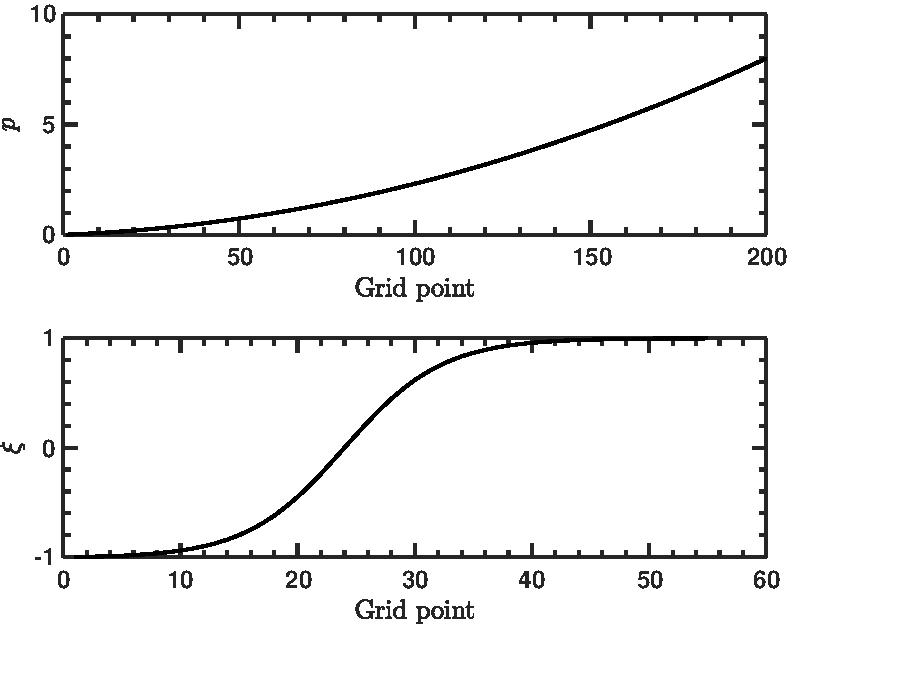
\includegraphics[width=12cm]{image63.pdf}
\caption{\label{fig:grid}网格p和ξ划分,其中动量空间p在[0 5]区间采用150个格点,在[5 10]动量空间采用50个格点,而$\xi$在区间[-1 -0.8]以及[0.8 1]区间采用30个格点,在[-0.8 0.8]区间采用了24个格点}
\end{figure}
由于非线性网格结构,微分方程\eqref{eq:diffstencil}需要稍作修正如下:
\begin{equation}
\frac{d f}{d p}=\frac{d f}{d s} \cdot\left(\frac{d p}{d s}\right)^{-1}
\end{equation}

\noindent 其中p为s的函数,s一般为[0  ,1]之间均匀格点,同样对于$ξ$也是同样处理,这时我们可以得到非线性网格点微分函数。下面我们通过一个简单的算例验证算法的精度,例如f=sin(x),$x=s^2$,$s=0:0.001:1$,求$df/dx$。分别用四阶差分格式和一阶差分格式计算,结果如\autoref{fig:error}所示,其中横坐标为x,纵坐标表示计算结果和理论值的相对误差的绝对值。计算结果表明:在ds=0.001的网格精度下使用一阶差分的相对精度约为$10^{-4}$,而四阶差分相对精度为$10^{-12}$,四阶差分比一阶差分精度高了约8个数量级,因此选择四阶差分用于数值计算具有更高的精度。
\begin{figure}[ht]
\centering
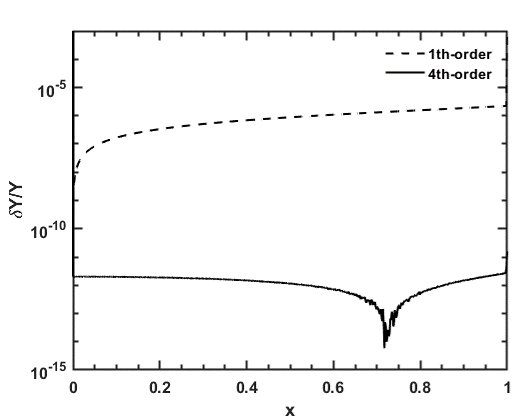
\includegraphics[width=10cm]{image64.png}
\caption{\label{fig:error}stencil微分方法一阶与四阶相对误差评估,$\frac{\delta Y}{Y}=\frac{abs(Y_{theory}-Y_{numerical})}{Y_{theory}}$表示理论解与数值解的相对误差}
\end{figure}\par
碰撞算符方程中的积分过程可使用matlab自带的梯形数值积分函数trapz或向量加权求和完成,至此,方程中系数和矩阵$C_{nm}$等求解均可得到解决。

\subsection{方程求解}
为了将动理学方程表示成可求解的矩阵形式,将方程\eqref{eq:Fnm} 写为大矩阵形式
\begin{equation}\label{eq:dFdt}
\frac{\partial F}{\partial \hat{t}}+M F=\hat{S}_{A}[F]
\end{equation}
其中$F=[F_0,F_1,…,F_N ]$为勒让德系数,这里选取有限的阶数N,通常N取40已经足够收敛。F元素个数为$(1,nP×nL)$,则M为$(nP×nL,nP×nL)$方矩阵,利用半隐式时间递推方法,上述方程可表示为:
\begin{equation}
F^{k+1}+\Delta t M^{k} F^{k+1}=\Delta t \hat{S}_{A}\left[F^{k}\right]+F^{k}
\end{equation}
利用标准的稀疏矩阵求逆的方法, 根据  $F^{k} $ 实现 $ F^{k+1} $ 求解, 即$  F^{k+1}=(I+   \left.\Delta t M^{k}\right)^{-1}\left(F^{k}+\Delta t \hat{S}_{A}\left[F^{k}\right]\right) $。 一般求解方程的主要困难是构造  $\mathrm{M} $ 矩阵, 当  $\mathrm{M} $ 矩阵和$F^k$有关时,每一次迭代过程中都需要更新M矩阵,因此高效解决M矩阵的更新是很重要的,这涉及到程序能否高效运行,能否在有限的计算机算力下完成相应计算任务,为了保持内容的连贯性,具体M矩阵构造过程可参考附录\autoref{sec:A6}。在程序设计中,这里首先将只需要计算一次的数据提前计算好,在时间的循环中迭代调用即可,这样可以避免大量的重复计算,提高计算效率。

在划分F网格中,动量p范围设置为$[0 ,p_{max}]$,网格划分如\autoref{fig:grid}所
示,在低能段p拥有更密的网格密度而高能段密度逐渐稀疏。勒让德阶数L范围为
 $\mathrm{L}=0: \mathrm{nL}-1$ , 阶数越高, 计算精度自然越高, 相应需要的计算
 时间越长, 通常取 $ \mathrm{nL}=40 $ 即可实现足够的计算精度。 $ \mathrm{p}=0  
 $处边界条件设置为 $ \frac{d F_{0}(0)}{d p}=0$, 当$\mathrm{L}>0$  时  $F_{L}(0)=0 $。 
 $p=p_{\max }$  处所有  $\mathrm{L} $ 均有$ F_{L}(p_{max})=0$  。为了避免在  $
 \mathrm{p}=p_{\max }  $由于强制为零导致数值在边 界出现非物理波动, 我们需
 要在边界添加额外的扩散方程以实现从边界到内部分 布函数的缓冲扩散, 扩散方
 程形式为 $c_{1} p^{-2} \partial / \partial p\left(p^{2} \exp \left(-\frac{\left[p-p_{\max }\right]}{c_{2}}\right) \partial F/ \partial p\right.$  ,通过 取合适的参数 $ c_{2}  
 $和  $c_{1}$  可以确保扩散方程只在边界有作用而不会影响内部, 这里取  $c_{1}
 =1$,$ c_{2}=1$ 。
\section{经典过程下电子能量分布函数演化的数值模拟}
\subsection{双温电子速度分布演化}
为了评估计算结果是否合理,我们构造这样一种场景:在均匀背景等离子体中存在两种热电子分布,其中温度$T_B$表示主体等离子体温度,温度$T_1$表示少量热电子温度。在这种条件下,我们研究温度$T_1$的少量热电子在背景温度$T_B$的热电子中速度分布演化过程。首先我们选取的模型中考虑电场项、Fokker-Plank碰撞项以及电子回旋辐射阻尼项。由于该模型中Fokker-Plank碰撞项是对分布函数的线性处理,在电子碰撞过程中,传递给背景电子的能量和动量并没有计算在内,因此这里不考虑背景电子温度的演化,计算中始终保持恒定值$T_B$。这样做只有在温度为$T_1$的电子数量$n(T_1)$远远小于背景热电子数$n(T_B )$的条件下成立。\par
考虑空间均匀分布,等离子体背景参数设置为:少量热电子温度$T_1=3KeV$,等离子体背景电子温度$T_B=1KeV$,背景电子密度$n_e=1×10^{19} m^{-3}$, 密度$n(T_1 )≪n_e$,电场强度$E=0 V/m$,背景磁场$B_0=0 T$,初始温度为$T_1$的热电子动理学方程为:
\begin{equation}\label{eq:Rad}
%\frac{\partial F}{\partial \hat{t}}+\widehat{\mathrm{E}}\left(\xi \frac{\partial F}{\partial p}+\frac{1-\xi^{2}}{p} \frac{\partial F}{\partial \xi}\right)+\hat{C}[F]+\frac{\partial}{\partial \boldsymbol{p}} \cdot \widehat{\boldsymbol{F}_{\mathrm{rad}}} F=0
\frac{\partial F}{\partial \hat{t}}+\hat{C}[F]=0
\end{equation}

将等离子体背景参数和初始条件作为程序的输入,取勒让德阶$nL=25$,$p_{max}$=4.8,$dt=7\times 10^{-5}s$,$t_{max}=4\times 10^{-3}s$,$nP=350$,边界吸收参数$c_1=0.01$,$c_2=0.01$,在Intel(R)Core™i7-10700CPU@2.90Ghz和24GB内存的电脑上运行约5s后完成所有计算,通过对F勒让德逆变换可得到$f(p,ξ)$随时间的演化,对$f(p,ξ)$中$\xi$变量积分得到$f_p=\int_{-1}^1f(p,\xi)\dif \xi$。
\begin{figure}[ht]
\centering
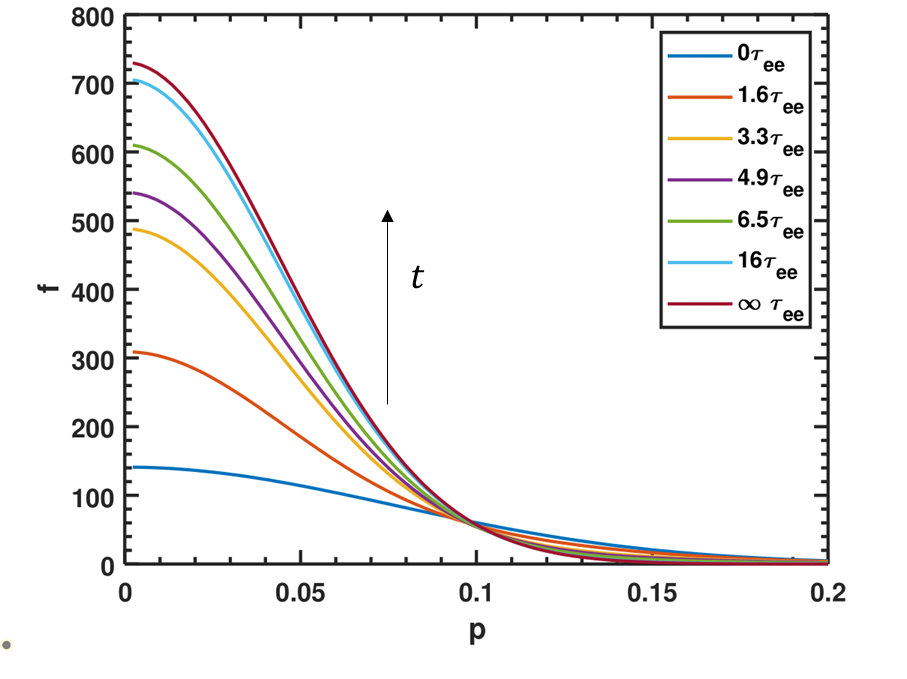
\includegraphics[width=10cm]{image65.png}
\caption{\label{fig:fevol}少量热电子的速度分布函数$f_p$随着慢化过程的演变,其中约化时间$\tau_{ee}=1/\nu_{ee}$,表示电子-电子碰撞周期.}
\end{figure}
\begin{figure}[H]
\centering
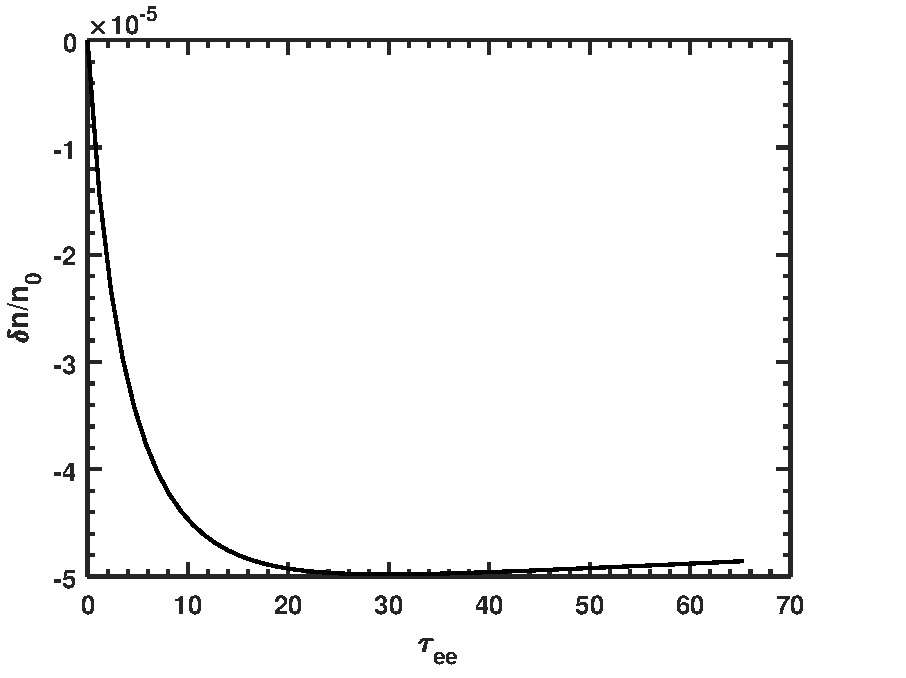
\includegraphics[width=12cm]{image66.pdf}
\caption{\label{fig:fneevol}相对密度变化量时序图}
\end{figure}
\par 如\autoref{fig:fevol}为不同时刻电子动量分布$f_p$图,从图中可以看出初始温度为3keV的热电子具有最大的分布展宽,随着和背景电子的碰撞,热电子的能量通过碰撞传递给背景电子使其自身的能量逐渐降低,导致$p=0$附近分布逐渐升高,分布函数展宽逐渐减小。忽略背景电子温度的升高,热电子的最终温度理论上应该等于1keV,而且在这个过程中,热电子的密度$n_e=∬f(p,ξ) p^2 2π\dif p\dif ξ=1$应始终保持守恒。\autoref{fig:fneevol}给出了密度相对变化量随时间的关系,其中$δn/n_0 =(n-n_0)/n_0$。理论上密度变化应该为零,但是由于数值的截断误差以及吸收边界条件,分布函数在边界会被吸收减小,导致在$60\tau_{ee}$内存在相对误差约$10^{-5}$。\autoref{fig:fevol2}给出了最初和最终热电子分布函数的形状以及背景温度为1keV的麦克斯韦分布。当分布函数演化到最终稳态分布时,在$p<0.2$部分分布函数基本和麦氏分布重合,但是$p>0.2$的形状高于麦氏分布,类似的现象在CODE模拟速度分布函数\cite{RN814}和RF电流驱动时Fork-Plank模拟中均有出现\cite{RN2067}。
附录\autoref{sec:NumCmp}中进一步展示了Pike碰撞模型和较为简化的Landreman碰撞模型计算结果对比,通过对等效温度的演化计算验证了两种模型的一致性。

\begin{figure}[H]
\centering
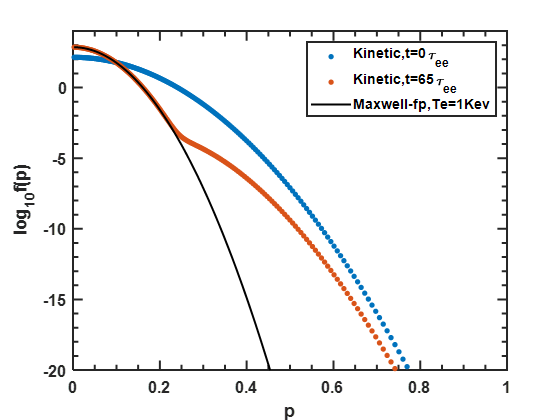
\includegraphics[width=12cm]{image67.png}
\caption{\label{fig:fevol2}分布函数的初始分布与最终分布以及$T_e=1KeV$的麦氏分布}
\end{figure}

\subsection{洛伦兹散射}
对于洛伦兹气体(例如铁,金属中的原子核形成周期性的矩阵网格,电子在它们之间自由运动,就像无限弹球一样),由于背景离子等效静止不动,在没有电场的环境中试探电子和背景离子碰撞电子始终保持能量守恒\cite{RN1839},只是运动方向逐渐趋向于各项同性,此时对应的动理学方程变为
\begin{equation}\label{eq:fLorz}
\frac{\partial \mathrm{f}}{\partial \hat{\mathrm{t}}}=v_{D} \frac{\partial}{\partial \xi}\left(1-\xi^{2}\right) \frac{\partial f}{\partial \xi}
\end{equation}
这里选取等离子体散射频率
\begin{equation}
v_{D}=\frac{3 \sqrt{\pi}}{4} \frac{\delta^{2} k_{e c}}{2 x p^{2}}\left[Z+\phi(x)-\Psi(x)+\frac{\delta^{4} x^{2}}{2}\right]
\end{equation}
将f表示为勒让德级数
\begin{equation}\label{eq:fleng}
f=A(\hat{t}) \sum_{L=0}^{\infty} F_{L}(p) P_{L}(\xi)
\end{equation}
将\autoref{eq:fleng}代入\autoref{eq:fLorz}得
\begin{equation}
\dot{A}(\hat{t}) \sum_{L=0}^{\infty} F_{L}(p) P_{L}(\xi)=-L *(L+1) \nu_D A(\hat{t}) \sum_{L=0}^{\infty} F_{L}(p) P_{L}(\xi)
\end{equation}
其解析解为
\begin{equation}
f=\sum_{L=0}^{\infty} F_{L}(p) P_{L}(\xi) * \exp \left(-L *(L+1) v_{D} \hat{t}\right)
\end{equation}
假设初始速度分布函数满足分布
\begin{equation}
f_{0}=\frac{1}{n_{0}} \exp \left(-\frac{\left(p_{\perp}-p_{\perp 0}\right)^{2}+\left(p_{\|}-p_{\| 0}\right)^{2}}{4 \Delta p^{2}}\right)
\end{equation}
取$p_{⊥0}=1$,$p_{∥0}=3$,$Δp=0.5$,$n_0$为$f_0$归一化常数。取$Lmax=22$,$dt=1\times 10^{-4}~s$,$p_{Max}=8$,nP=350。在温度T=1~KeV,密度$n=1×10^{19}~ m^{-3}$,有效电荷数Z=1,磁场强度B=0~T的背景中分布函数的理论和数值结果如\autoref{fig:lorzen}所示,其中(a)图为初始速度分布,(b)图为根据方程计算出的解析解,(c)图为数值解,(d)图为精确解和数值的相对误差,通过(数值解-解析解)/解析解的最大值*100得到,由此可见在该模型下数值计算的相对误差约为$10^{-5}$。\autoref{fig:errornega}展示了数值求解下密度和平均能量的时序图,该系统散射频率约为$ν=ν_D*ν_{cc} \approx 0.283~s^{-1}$,至少需要3.5~s才能达到平衡状态,在系统达到平衡的过程中,算法能够提供足够好的守恒性和稳定性。
\begin{figure}
\centering
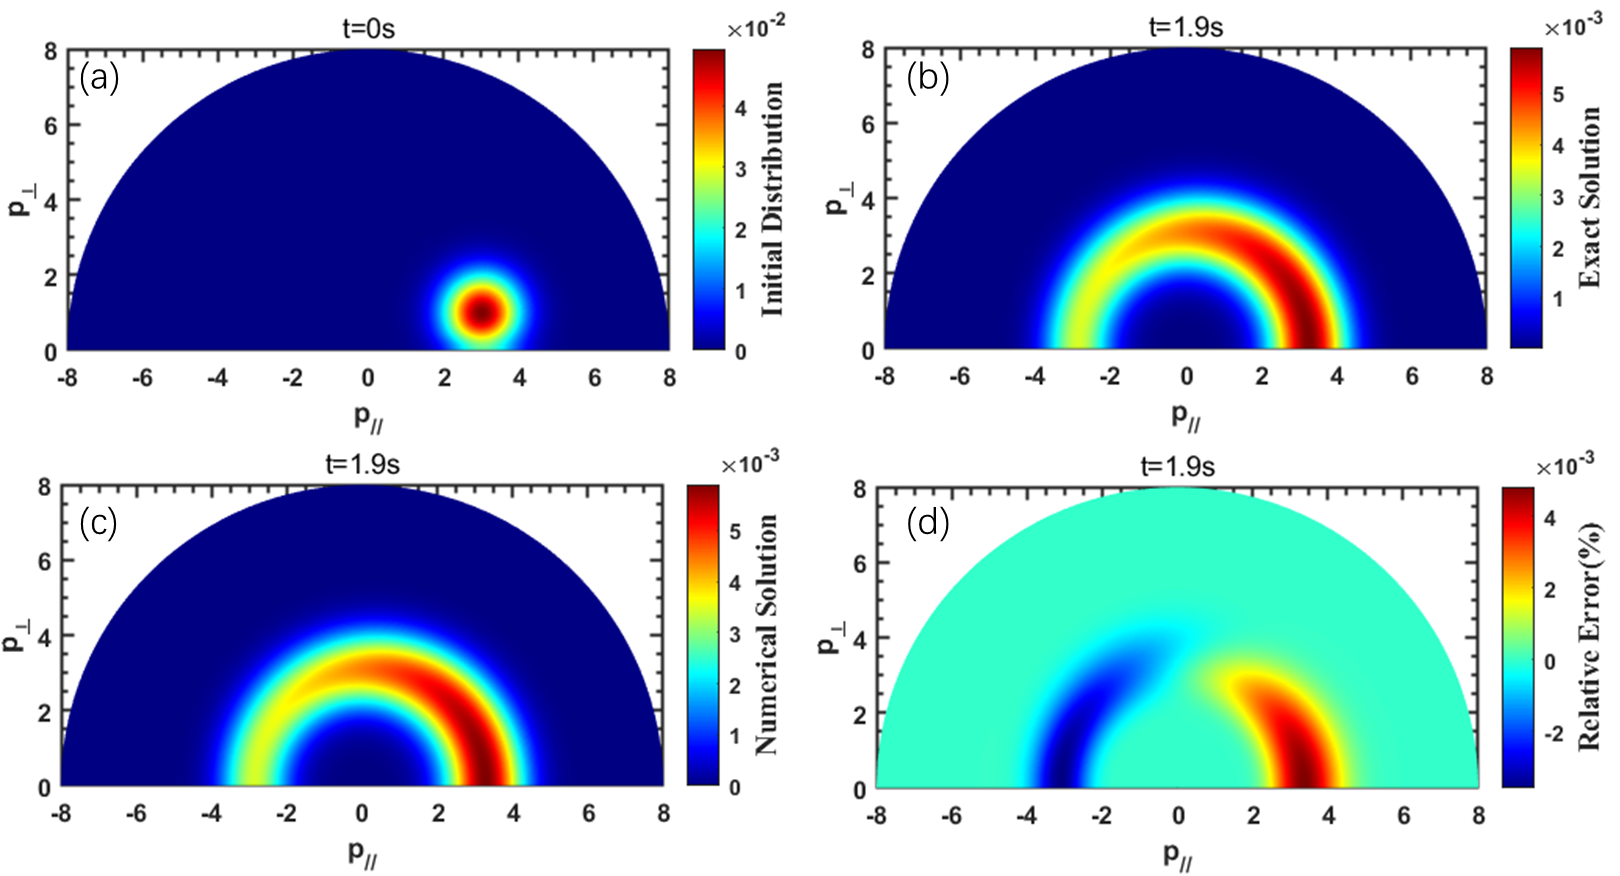
\includegraphics[width=12cm]{image70.png}
\caption{\label{fig:lorzen}分布函数演化和相对误差,(a)初始速度分布(b)t=1.9s时速度分布的理论解(c)t=1.9s时速度分布的数值解(d)数值和理论的相对误差}
\end{figure}\par


\begin{figure}
\centering
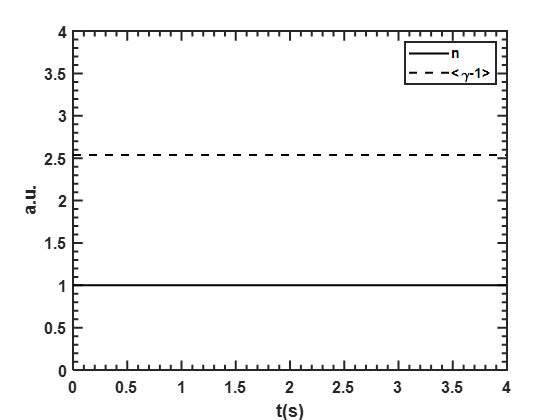
\includegraphics[width=12cm]{image71.png}
\caption{\label{fig:errornega}数值解的密度和平均能量时序图}
\end{figure}\par

\subsection{强磁场下速度分布演化}

如前文所述,匀强磁场背景中电子受电场驱动会不断加速,同时辐射阻尼也在增加,当辐射阻尼力和电场力平衡时,电子达到最大速度,电子速度不再增加。这里我们通过动理学方程模拟如上过程用以测试程序计算结果是否合乎逻辑。
为了减少计算空间,加快计算效率,这里取磁场强度B=8~T,电场强度E=0.008~V/m,背景电子温度为10~keV,电子密度为$0.1\times10^{19}~m^{-3}$。为了让大部分电子都能逃逸,这里设置电子初始分布具有60~keV的麦氏分布。 \autoref{fig:Bfevo}(a)为计算结果趋于稳定状态下的电子速度分布图,主要存在两个区间,分别是低能区间的热分布以及逃逸区间的非热分布,逃逸区间的电子受到辐射阻尼导致速度不能无限增加,最终在稳定点附近聚集。\autoref{fig:Bfevo}(b)为试探粒子速度相空间演化以及流场图(可参考附录\autoref{sec:A5},最终运动方程是通过动理学方程推导得到),从速度相空间演化可以看出在$q_∥\sim7.9$,$q_⊥\sim0.56$处存在吸引子,该点为逃逸电子的最终速度,而流场矢量大小告诉我们不同空间位置处速度变化率,可以看出在吸引子附近速度变化率都很小,这可能是\autoref{fig:Bfevo}(a)中的分布主要在吸引子左侧附近的原因,因为主体分布越靠近吸引子变化越缓慢,越靠近受力平衡点,电子的加速度越小。\par

关于吸引点准确位置,可以通过联立试探粒子运动方程组得到,试探粒子运动方程为(参考附录\autoref{sec:A5})
\begin{align}\frac{\partial p_{\parallel}}{\partial \tau} & = \frac{p \xi\left(1-\xi^{2}\right)}{\gamma k}-\frac{\gamma p\left(1-\xi^{2}\right) \xi}{k}-2 p \xi K+D_{\parallel}+\hat{E} \\\frac{\partial p_{\perp}}{\partial \tau} & = \frac{-p \xi^{2}\left(1-\xi^{2}\right)^{\frac{1}{2}}}{\gamma k}-\frac{\gamma p\left(1-\xi^{2}\right)^{\frac{3}{2}}}{k}+\frac{p\left(2 \xi^{2}-1\right)}{\sqrt{1-\xi^{2}}} K+D_{\perp}\end{align}
当试探粒子受力平衡时,即为吸引点位置,此时
\begin{align}\frac{p \xi\left(1-\xi^{2}\right)}{\gamma k}-\frac{\gamma p\left(1-\xi^{2}\right) \xi}{k}-2 p \xi K+D_{\parallel}+\hat{E} & = 0 \\\frac{-p \xi^{2}\left(1-\xi^{2}\right)^{\frac{1}{2}}}{\gamma k}-\frac{\gamma p\left(1-\xi^{2}\right)^{\frac{3}{2}}}{k}+\frac{p\left(2 \xi^{2}-1\right)}{\sqrt{1-\xi^{2}}} K+D_{\perp} & = 0\end{align}
通过求解上方程组得到平衡点为(7.91,0.561),与图中结果一致
\begin{figure}[ht]
\centering
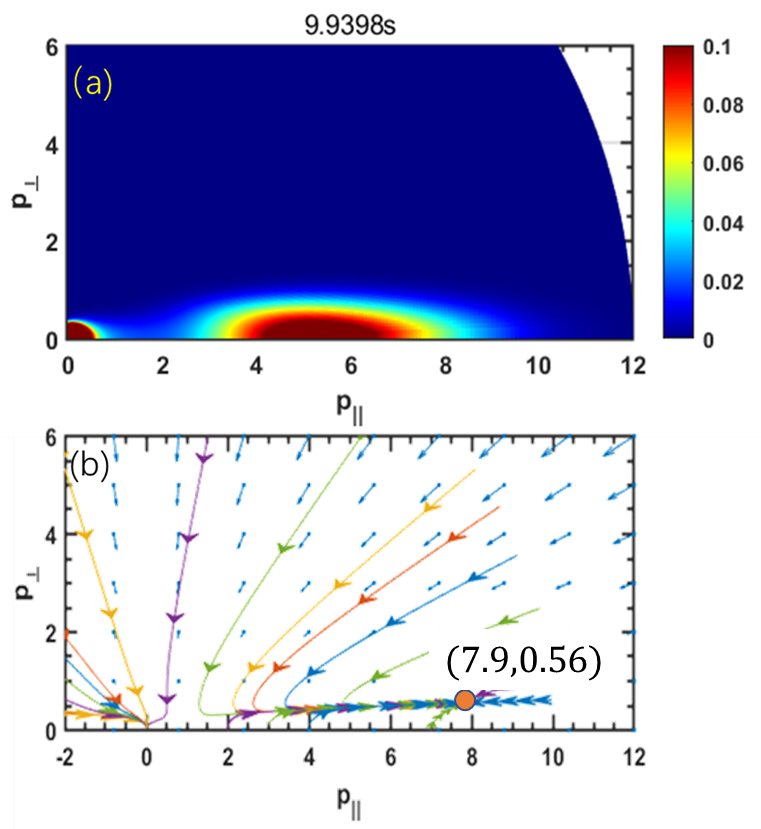
\includegraphics[width=12cm]{image72_1.png}
\caption{\label{fig:Bfevo}(a)趋于稳定状态下的速度分布(b)流场图以及试探粒子速度相空间轨迹}
\end{figure}

\vspace{3\baselineskip}

\subsection{雪崩电子}
逃逸电子产生后会和背景电子发生大角度碰撞,此时原先的逃逸电子也会因为碰撞速度发生改变。当碰撞后的背景电子速度超过逃逸速度临界阈值时就会发展成新的逃逸电子,该效应称为雪崩效应,该效应产生的新的逃逸电子称为雪崩电子。
\par 如\autoref{fig:avavec}(a)所示,碰撞过过程电子满足能量守恒和动量守恒\cite{RN1941},
\begin{figure}[ht]
\centering
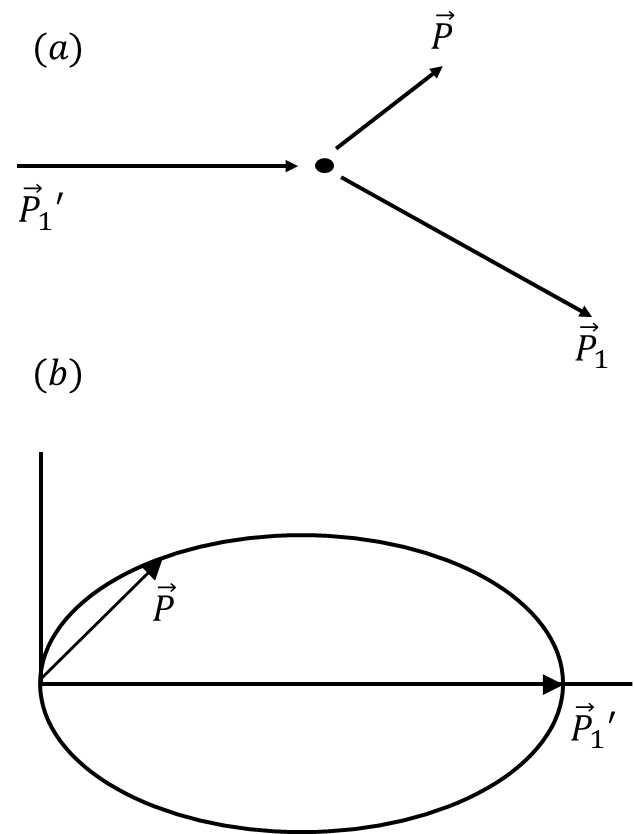
\includegraphics[width=7cm]{image73_1.png}
\caption{\label{fig:avavec}(a)逃逸电子与背景电子碰撞导致的大角度散射(b)结合动量守恒和能量守恒得到的散射动量椭圆关系
}
\end{figure}
 根据
\begin{align}
\gamma_{1}^{\prime} & = \gamma_{1}+\gamma-1 \\
{\vP_{1}^{\prime}} & = {\vP_{1}}+{\vP}
\end{align}
得到
\begin{equation}
\frac{P_{\perp}^{2}}{2\left(\gamma_{1}^{\prime}-1\right)}+\left(\frac{P_{\|}}{\left(\gamma_{1}^{\prime 2}-1\right)^{\frac{1}{2}}}-\frac{1}{2}\right)^{2}=\frac{1}{4}
\end{equation}
其中$\gamma=\sqrt{1+P^{2}}$,该方程对应的椭圆曲线如\autoref{fig:avavec}(b)所示,
利用该方程可得到碰撞后新产生的电子逃逸角为\cite{RN1811,RN1809}
\begin{equation}
\xi=\sqrt{\frac{(\gamma-1)\left(\gamma_{1}{ }^{\prime}+1\right)}{(\gamma+1)\left(\gamma_{1}{ }^{\prime}-1\right)}}
\end{equation}
当入射的逃逸电子平行于磁场运动时,最大动量为$p_{max}$对应的最小碰撞散射角为
\begin{equation}
\xi_{\min }=\sqrt{\frac{(\gamma-1)\left(\gamma_{\max }{ }^{\prime}+1\right)}{(\gamma+1)\left(\gamma_{\max }{ }^{\prime}-1\right)}}
\end{equation}
其中$γ_{max}=\sqrt{1+p_{max}^2 }$。如\autoref{fig:avafig2}所示,其中黑色虚线即表示$ξ_{min}$,由于实际计算中我们同时考虑了逃逸电子的速度分布和角度分布,因此在$ξ_{min}$两侧都存在碰撞散射角,图中白色虚线为正负边界线,负区域表示电子速度损失区域,包含被碰撞的背景热电子以及逃逸电子,正区域为雪崩电子,即碰撞后的逃逸电子和新产生的逃逸电子,半圆形的白色虚线为逃逸临界速度曲线。
\begin{figure}
\centering
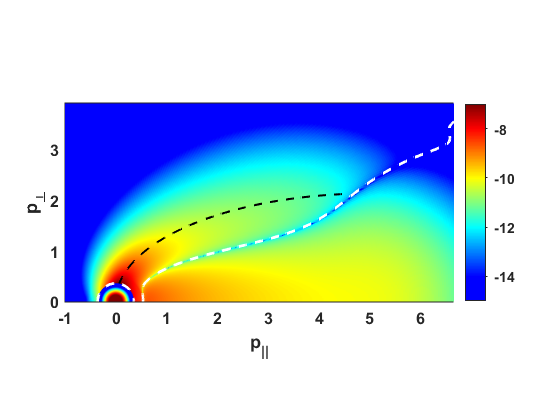
\includegraphics[width=11cm]{image74.png}
\caption{\label{fig:avafig2}大角度碰撞过程展示,其中白色为正负分界线,白色虚线以下的区域(包括半圆区域和右侧区域)为负,白色以上区域为正,黑色虚线为$ξ_{min}$}
\end{figure}
\subsection{程序校验}
不考虑角度分布条件下, 逃逸电子的速度阈值为 $ p_{c}=\frac{1}{\sqrt{\hat{E}-1}}\left(\hat{E}=\frac{E}{E_{C}}, E_{C} \text{表示} Connor \text{电场 }\right)$  。逃逸电子增长率 $ \gamma=\frac{1}{n} \frac{d n_{r}}{d t}  $作为方程计算中重要的参数, 可用于程序和程序之间互相校验的标准。
   
将分布函数用勒让德函数展开后, 勒让德零阶系数表示密度分布, 逃逸电子 增长率可表示为:
\begin{equation}
\gamma=\frac{1}{n} \frac{d n_{r}}{d \hat{t}}=\int_{p_{b}}^{\infty} \frac{\partial f}{\partial \hat{t}} 4 \pi p^{2} d p=\int_{p_{b}}^{\infty} \frac{\partial F_{0}}{\partial \hat{t}} 4 \pi p^{2} d p
\end{equation}
其中  $f=\sum_{0}^{N} F_{L}(p) P_{L}(\xi) $, 积分下边沿$p_{b}$  可取 $ 5 p_{c}$ 。根据方程 \eqref{eq:dFdt}, $\frac{\partial F_{0}}{\partial \hat{t}}=\left(\hat{S}_{A}[F]-M F\right)_{0}$, 在不考虑雪崩效应时,由于电子在 $ \left[5 p_{c}, 20 p_{c}\right] $ 之间既没有源项也没有损失项, 因此 $ p_{b} $在该区间的 取值对计算结果几乎没有影响,这样计算所得为初级逃逸电子增长率。最后初级逃逸电子增长率可表示为
\begin{equation}\label{eq:runrate}
\gamma=\int_{p_{b}}^{\infty}\left(-M F\right)_{0} 4 \pi p^{2} d p
\end{equation}

过去的这些年中,有很多作者发展了自己的计算程序用来分析逃逸电子,为了确保自己的程序准确无
误,我们将以逃逸电子增长率为标尺,通过和前人计算同一个物理参数下的逃逸电子增长率来鉴定程序的准确度,这里我
们以1973年普林斯顿大学Kulsrud在PRL发表的论文\cite{RN2095}	为参考对象。 \autoref{fig:runrate}为
自主开发程序Kinetic和Kulsrud在非相对论条件下$(δ→0)$初级逃逸电子增长率计算结果的对比图,
可以看出二者计算结果完全一致。其中本文中逃逸电子增长率采用背景温度为0.5keV,对应
$δ=4.4×10^{-2}$。逃逸电子增长率计算采用方程\eqref{eq:runrate},对应的$p_b=5*p_c$。需要注意
的是在本图坐标系下, Kulsrud 论文中 table  1表格的约化电场和增长率 需要相应变换: $ \hat{E}
=\hat{E}_{k} * \frac{3 \sqrt{\pi}}{2}$,$ \gamma=\gamma_{k} 3 \sqrt{\frac{\pi}{2}} $ 。这是因为 $ 
Kulsrud $ 采用的约化电场 $ E_{\text {Kulsrud }}=\frac{2}{3 \sqrt{\pi}} \frac{E}{E_{D}} $, 约化时间  
$v_{K}=3 \sqrt{\frac{\pi}{2}} v_{e e}$ , 其中  $v_{e e}  $为电子-电子碰撞频率,  $E_{D}=   \frac{m_{e} 
v_{e e} v_{T e}}{e}  $。
\begin{figure}[H]
\centering
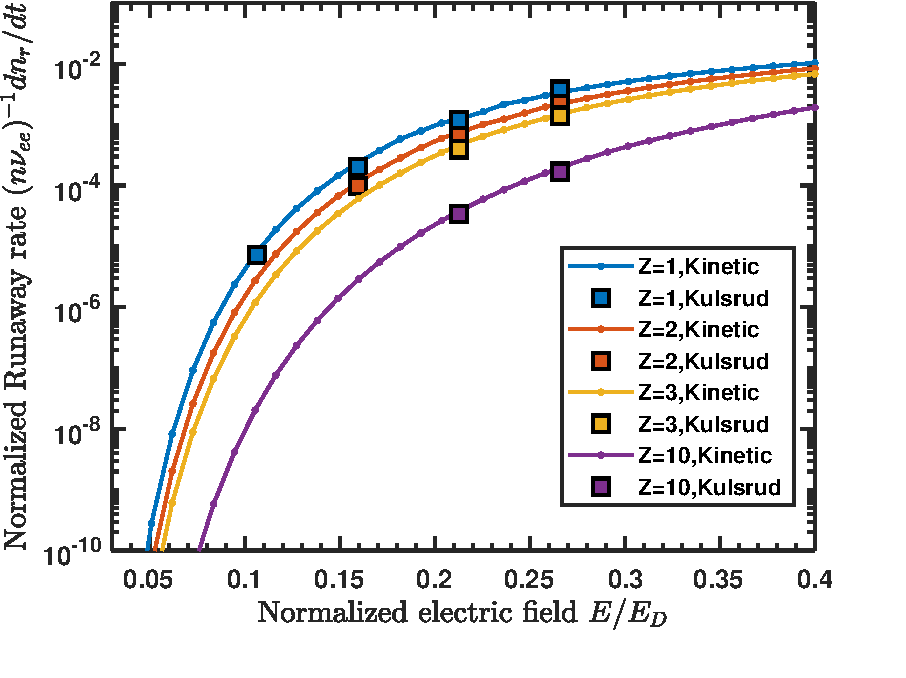
\includegraphics[width=12cm]{image75.pdf}
\caption{\label{fig:runrate}非相对论条件下逃逸电子增长率Kinetic 程序和Kulsrud在table 1\cite{RN2095}	中计算结果,Z表示等离子体中离子有效电荷数}
\end{figure}

\section{均匀电磁场中电子与电磁波的相互作用}\label{sec:ewmele}
以上我们讨论了静磁场环境中电子速度分布在外界电场驱动下的动理学演化过程,但是我们忽略了其中重要的一项——电磁湍动项。当逃逸电子产生时,逃逸电子和磁化等离子体本征模通过波粒相互作用激发出本征波,如哨声波、非寻常波等,激发出的电磁波又进一步和逃逸电子相互作用导致逃逸电子出现速度散射。电磁波和电子相互作用的过程称为电磁湍动\cite{胡希伟2006等离子体理论基础}。从动理学方法求解这个过程涉及到两个过程,首先需要根据波的增长率计算波的能量随时间的变化(\autoref{eq:gammab}),然后求解湍动算符(\autoref{eq:emwdiffuse})。目前主要问题是在计算\autoref{eq:emwdiffuse},谱方法和湍动算符似乎有着不可调和的矛盾,将湍动算符用谱方法展开后无法实现高效计算。面对这样的问题,我们选择了一条简化的方法:不考虑电磁波的激发,只考虑电磁波和单电子的相互作用,从单电子的角度研究电磁波和电子的相互作用过程。
\par 磁化等离子体电子与电磁波或静电波相互作用主要通过三种共振机制实现能量交换,分别是多普勒共振(Normal Doppler Effect,NDE)、切伦科夫共振以及反常多普勒共振(Anomalous Doppler Effect, ADE)。其中多普勒共振是电子回旋共振加热以及电子电流驱动主要物理机制。切伦科夫共振主要表现在静电波与电子相互作用,也称为朗道共振。朗道共振过程中,粒子在波场运动如同冲浪,该机制会导致速度分布函数在共振点被拉平,形成共振平台\cite{RN1801}。反常多普勒效应会导致电子平行方向速度散射到垂直方向并释放出电磁波。本节通过经典电动力学模拟单电子与电磁波的三种共振机制,从经典力学中理解ADE的物理过程,然后通过分析冷等离子体中电磁波本征模和ADE产生条件,对通过主动注入电磁波实现抑制逃逸电子的可能性进行了探讨。
\subsection{单电子与电磁波相互作用数值模拟}\label{sec:simulationVPA}
根据反常多普勒效应的量子解释(\autoref{sec:quantum}),对于以速度$v_z$沿匀强磁场运动的电子回旋系统,系统存在三种共振频率:多普勒频率、Cerenkov频率和反常多普勒频率。我们只考虑$n=0\text{,}±1$(它们是最主要的共振阶数),那么这些频率分别为
\begin{equation}\label{eq:resonant}
\begin{aligned}\omega_{N D E} & = k \cos (\theta) v_{z}+\omega_{c e} \\\omega_{\text {Cerenkov }} & = k \cos (\theta) v_{z} \\\omega_{A D E} & = k \cos (\theta) v_{z}-\omega_{c e}\end{aligned}
\end{equation}
从量子角度上看,如果背景中存在具有共振频率的诱导波,电子回旋系统将会受激发射光子或受激吸收光子,导致系统内能和动量产生相应的变化。为了从经典电动力学理解该物理过程,我们设计了如下模型:

考虑均匀磁场$B_0=B_z$ 背景中存在平行与磁场并与磁场方向反向的均匀电场$E_0$,同时背景还存在频率为ω,波数为k的稳态电磁波,其中k与z轴的夹角为θ,如\autoref{fig:waveset}所示。初始电子为静止状态,随着静电场的加速,电子的速度不断增大, $ω_{NDE}$ 、$ω_{Cerenkov}$以及$ω_{ADE}$共振频率也在不断升高。当共振频率升高到和背景电磁波频率相同时,电子回旋系统即处于“受激状态”,出现“能量跃迁”,这样我们就可以研究该过程中电子的运动变化。

\begin{figure}
\centering
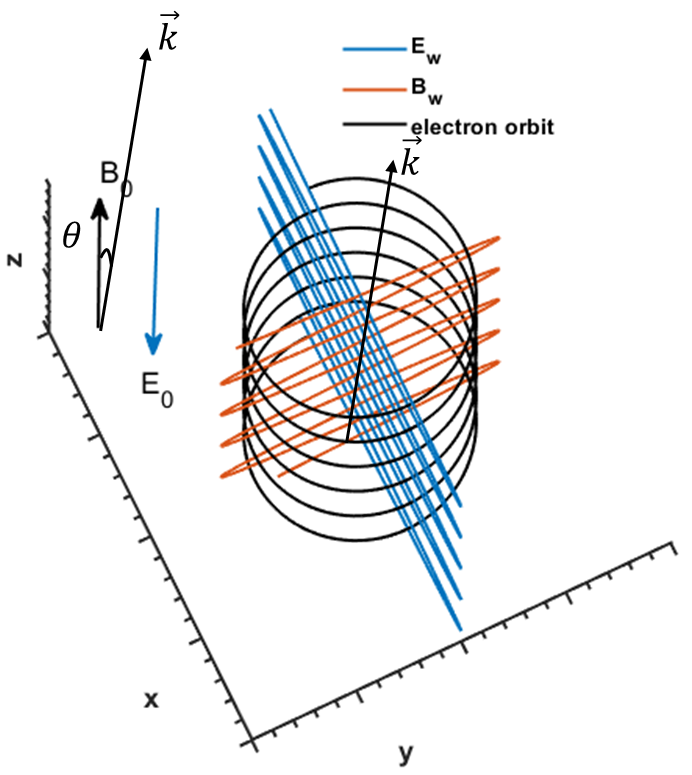
\includegraphics[width=7cm]{image76.png}
\caption{\label{fig:waveset}ADE模拟背景参数设置}
\end{figure}
考虑相对论效应电子运动方程为:
\begin{equation}\label{eq:motion}
\begin{aligned}
\frac{\mathrm{d} \mathbf{x}}{\mathrm{d} t} & = \frac{\mathbf{p}}{\sqrt{m_{0}^{2}+\mathbf{p}^{2} / c^{2}}} \\\frac{\mathrm{d} \mathbf{p}}{\mathrm{d} t} & = q\left(\mathbf{E}(\boldsymbol{x}, \boldsymbol{t})+\frac{\mathbf{p}}{\sqrt{m_{0}^{2}+\mathbf{p}^{2} / c^{2}}} \times \mathbf{B}(\boldsymbol{x}, \boldsymbol{t})\right)
\end{aligned}
\end{equation}
这里$𝑬$和B是静态场和电磁波(EMW)中电场分量和磁场分量之和,$𝑝=𝛾𝑚_e𝑣$。
电子运动方程的数值求解通常采用Boris算法\cite{RN2016},但这里我们采用保体积算法(VPA)\cite{RN1907},因为保体积算法相对于Boris算法能够在更长的计算时间保持数值精度 。通过使用VPA算法,微分方程\eqref{eq:motion} 的离散结构可以写为
\begin{equation}
\left\{\begin{array}{l}\mathbf{x}_{k+\frac{1}{2}}=\mathbf{x}_{k}+\frac{\Delta t}{2} \frac{\mathbf{p}_{k}}{\sqrt{m_{e}^{2}+\frac{\mathbf{p}_{k}^{2}}{c^{2}}}}, \\\mathbf{p}^{-}=\mathbf{p}_{k}+q \frac{\Delta t}{2} \mathbf{E}_{k+\frac{1}{2}}, \\\mathbf{p}^{+}=\text {Cay }\left(\frac{q \Delta t \hat{B}_{k+\frac{1}{2}}}{2 \sqrt{m_{e}^{2}+\frac{\mathbf{p}^{-2}}{c^{2}}}}\right) \mathbf{p}^{-}, \\\mathbf{p}_{k+1}=\mathbf{p}^{+}+q \frac{\Delta t}{2} \mathbf{E}_{k+\frac{1}{2}}, \\\mathbf{x}_{k+1}=\mathbf{x}_{k+\frac{1}{2}}+\frac{\Delta t}{2} \frac{\mathbf{p}_{k+1}}{\sqrt{m_{e}^{2}+\frac{\mathbf{p}_{k+1}^{2}}{c^{2}}}},\end{array}\right.
\end{equation}
其中 Cay 表示 Cayley 变换, 具体方法可参考文献\cite{RN1907}。 对方程无量纲化:  $p^{*}=   \frac{p}{m_{e} c}, B^{*}=\frac{B}{\frac{m_{e}}{e \tau_{c e}}}, E^{*}=\frac{E}{\frac{E}{\tau_{e e} c}}, \Delta t^{*}=\frac{\Delta t}{\tau_{c e}}, x^{*}=\frac{x}{\tau_{c e} c} $, 其中$  \tau_{c e} $ 表示电子回旋周期, $ m_{e}  $表示静电子质量, 原式化为
\begin{equation}
\begin{array}{l}\left\{\begin{array}{l}\mathbf{x}_{k+\frac{1}{2}}^{*}=\mathbf{x}_{k}^{*}+\frac{\Delta t^{*}}{2} \frac{\mathbf{p}_{k}^{*}}{\gamma_{\mathrm{k}}}, \\\mathbf{p}^{*-}=\mathbf{p}_{k}^{*}+\frac{\Delta t^{*}}{2} \mathbf{E}_{k+\frac{1}{2}}^{*}, \\\mathbf{p}^{*+}=\operatorname{Cay}\left(\frac{\Delta t^{*} \widehat{B}^{*}{ }_{k+\frac{1}{2}}}{2 \gamma^{*-}}\right) \mathbf{p}^{*-} \\\mathbf{p}_{k+1}^{*}=\mathbf{p}^{*+}+\frac{\Delta t^{*}}{2} \mathbf{E}_{k+\frac{1}{2}}^{*}, \\\mathbf{x}_{k+1}^{*}=\mathbf{x}_{k+\frac{1}{2}}^{*}+\frac{\Delta t^{*}}{2} \frac{\mathbf{p}_{k+1}^{*}}{\gamma_{\mathbf{k}+1}},\end{array}\right.\end{array}
\end{equation}
其中$\widehat{B}*$表示为
\begin{equation}
\widehat{B^{*}}=\left(\begin{array}{ccc}0 & B_{z}^{*} & -B_{y}^{*} \\-B_{z}^{*} & 0 & B_{x}^{*} \\B_{y}^{*} & -B_{x}^{*} & 0\end{array}\right)
\end{equation}
为了减少模型的复杂度,避免额外物理过程的干扰,首先我们选取的是线偏振电磁波(任意传播方向下偏振光的函数表达式可参考附录\autoref{sec:A7})。 取  $\theta=   0$, $\mathrm{k}=10^{5} / \mathrm{m}$ ,为了缩短计算时间, 这里取 $ B_{0}=200~ G s$, $\omega=1.5 \omega_{c 0}$ , 其中  $\omega_{c 0} $ 表示电子回旋频率,  $\omega_{c 0}=\mathrm{eB} / \mathrm{m}_{\mathrm{e}}$ , 静电场  $E_{0}=-2.5 \mathrm{ V} $, 静电场方向与 $ \mathrm{B}_{0} $ 反向。电子初始时刻速度为零, 电磁波电场强度为$  E_{p}=9~ \mathrm{ V} / \mathrm{m} $。 为 了保证计算收敛, 同时提高计算效率, 我们取时间步长为: $ \Delta t=\min \left(\frac{2 \pi}{50(k \cdot v)}\right.$ , $ \left.\frac{2 \pi}{50 \omega},\frac{2 \pi}{50 \omega_{c 0}}\right)$ , 这样可以保持电子空间中电磁波单位步长内相角变化不超过$  \pi / 25$ ,也可以保证电子运动一个波长内至少存在50个数值计算点。\par 计算结果如\autoref{fig:orbit}所示,
\begin{figure}[ht]
\centering
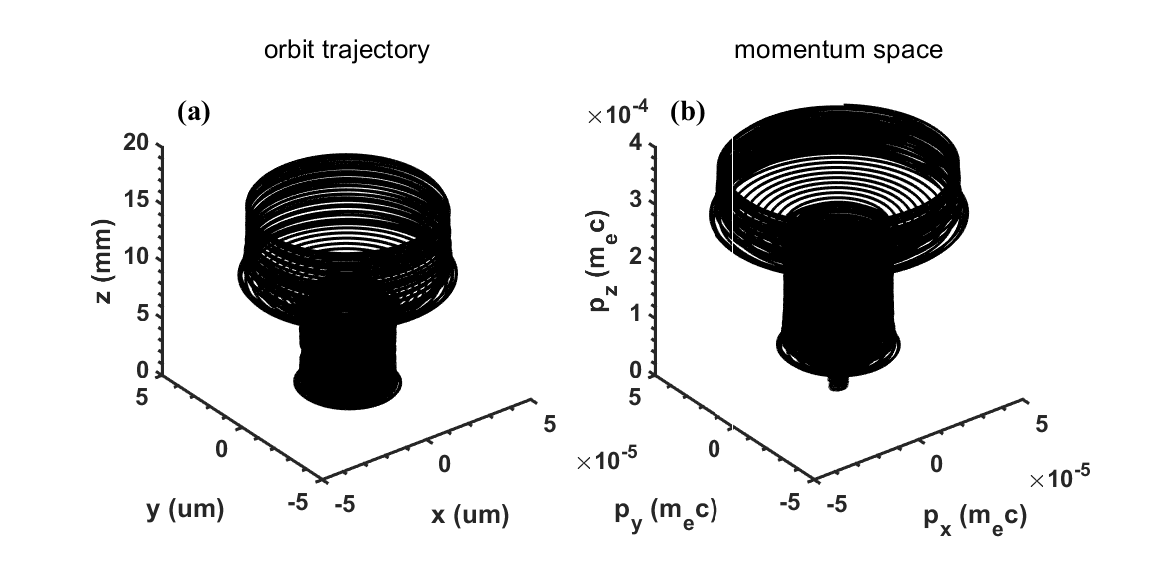
\includegraphics[width=12cm]{image77_1.eps}
\caption{\label{fig:orbit}(a)电子轨道图(b)电子动量空间图
}
\end{figure}
根据电子轨道图(\autoref{fig:orbit}(a))以及电子动量空间(\autoref{fig:orbit}(b))图
可以看出:电子在加速过程中存在两次垂直方向速度快速增加。
\autoref{fig:adepars}展示了电子运动过程中的各物理量的演化,随着电子平行方
向速度不断增加(\autoref{fig:adepars}(a)),多普勒频率$\omega_{NDE}$首先增
加到电磁波频率(\autoref{fig:adepars}(b),$τ=23τ_{ce}$),此时电子与
电磁波产生多普勒共振,垂直方向速度迅速变大(\autoref{fig:adepars}(d),$τ=23τ_{ce}$),同时电磁波对平行方向电子做
功为正(\autoref{fig:adepars}(c),$τ=23τ_{ce}$)。这就相当于电子受激吸收光子,电子平行方向和垂直方向速度均增加。根据量子分析(\autoref{sec:quantum}),对于多普勒共振,当系统发射光子会消耗系统内能和动能。以上过程相当于系统吸收光子,导致系统内能和动能增加。吸收光子和发射光子互为逆过程。
\par 当电子速度进一步增加,多普勒频率$\omega_{NDE}
$继续升高,多普勒共振频率超过了背景电磁波频率,因此多普勒共振现象消失。当时间来到$τ=132τ_{ce}$时,反常多普勒频率$\omega_{ADE}$达到与电磁波频
率相同,电子再次和电磁波共振,此时可以看到电子垂直方向速度再次迅速增大
(\autoref{fig:adepars}(d)),电磁波在平行方向对电子的功为负
(\autoref{fig:adepars}(c)),电子平行方向损失能量。这个过程类似量子理论中电
子受激发射光子,导致电子损失平行方向动能转化为垂直方向回旋内能。
\begin{figure}
\centering
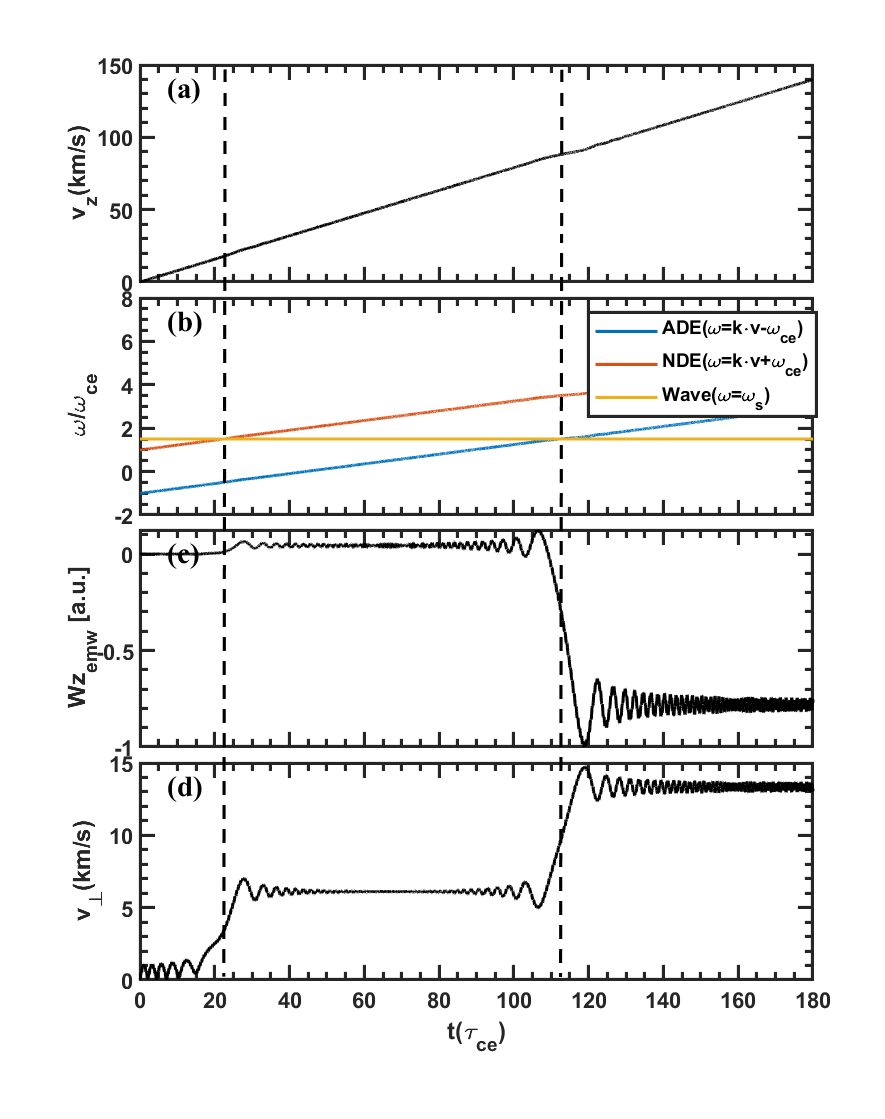
\includegraphics[width=11cm]{image78.eps}
\caption{\label{fig:adepars}参数演化图:(a)平行速度(b)多普勒频率($
\omega_{NDE}$)、反常多普勒频率($\omega_{ADE}$)随时间的演化(c)平行
方向电磁波对电子的功(可参考\autoref{sec:force}中电子在电磁波中的受力分析)(d)垂直速度
}
%

\end{figure}
如\autoref{fig:RLade}所示,当我们进一步将线极化波分解为左旋圆极化波和右旋
圆极化波时,我们发现右旋极化波对应多普勒共振,而左旋圆极化波只对应反常
多普勒共振。

\begin{figure}
\centering
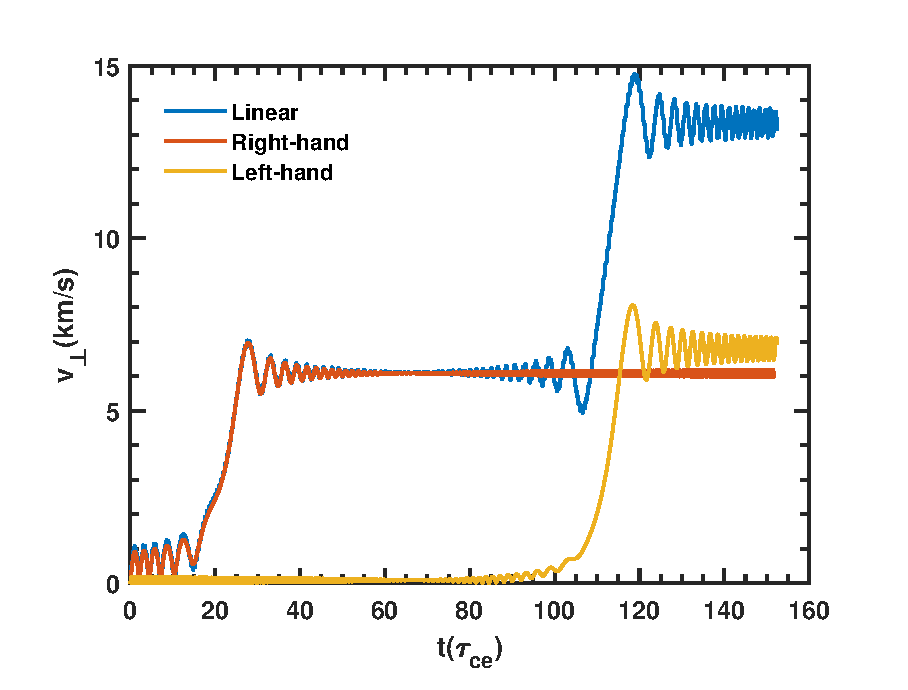
\includegraphics[width=12cm]{image79.eps}
\caption{\label{fig:RLade}不同极化电磁波对电子垂直速度的影响.其中左旋圆极化波只产生ADE作用($t\sim113\tau_{ee}$),而右旋圆极化波只产生NDE作用($t\sim22\tau_{ee}$).
}
\end{figure}

\subsection{ADE与电磁波的偏振}
首先共振发生时,取相对电子运动导心静止的参考系,该参考系相对实验室坐标系以电子平行方向速度$v_z$运
动。在该参考系中电磁波频率和电子的旋转频率一致,电磁波的频率和波
数分别为$ω'$和$k'$(ω和k分别为实验室坐标系下电磁波的频率和波数),根据洛
伦兹变换,实验室坐标系和相对静止坐标系的电磁波参数由如下方程连接:
\begin{equation}
\left[\begin{array}{c}
{\vk} \\
\frac{\omega}{c}
\end{array}\right]=\left[\begin{array}{cc}
\bar{\bar{\alpha}} & +\gamma {\vec{\beta}} \\
+\gamma {\vec{\beta}} & \gamma
\end{array}\right]\left[\begin{array}{c}
{\vk}^{\prime} \\
\frac{\omega^{\prime}}{c} 
\end{array}\right]
\end{equation}
其中  $\vec{k}=k_{x} \overrightarrow{e_{x}}+k_{y} \overrightarrow{e_{y}}+k_{z} 
\overrightarrow{e_{z}}\left(\overrightarrow{k^{\prime}}=k_{x}^{\prime} 
\overrightarrow{e_{x}}+k_{y}^{\prime} \overrightarrow{e_{y}}+k_{z}^{\prime} 
\overrightarrow{e_{z}}\right) $ 和$ \omega\left(\omega^{\prime}=\omega_{c 0}
\right)  $, $  \vec{\beta}=\frac{\vec{v}}{c}$ , $\gamma=\frac{1}
{\sqrt{\left(1-\beta^{2}\right)}} $ 是洛伦兹因子, $ \bar{\bar{\alpha}}=I+
(\gamma-1) \frac{\vec{\beta} \vec{\beta}}{\beta^{2}} $, 其中 I 为单位张量。通过
洛伦兹变换, 我们得到:
\begin{equation}
\begin{aligned}\omega & =\gamma \omega_{c 0}+\gamma v k_{z}^{\prime} \\
k_{z} & =\gamma k_{z}^{\prime}+\gamma \frac{v}{c} \frac{\omega_{c 0}}{c}
\end{aligned}
\end{equation}
$\text { 其中 } k_{z}=\frac{\omega}{c^{\prime} \cos (\theta)} \text {, 代入上述方程
得: }$
\begin{equation}
\omega=\frac{\omega_{c e}}{1-\frac{v}{c^{\prime}} \cos (\theta)}
\end{equation}
其中$  \omega_{c e}=\frac{\omega_{c 0}}{\gamma} $。频率$\omega$和$\omega_{ce}$的正负关系分别对应两种共振状态:(1) 多普勒共振, 根据共振
方程\eqref{eq:resonant}	可知 $ v_{N D E}=   \frac{\omega-\omega_{c 0}}{k_{z}}
$,$ \frac{v_{N D E}}{c^{\prime}} \cos (\theta)<1$, $\omega $ 和  $\omega_{c 0} $ 
符号相同, 具有同向旋转的物理特征, 因此多 普勒共振波具有右旋波特征。(2) 反
常多普勒共振, 根据共振方程可知 $ v_{A D E}=\frac{\omega+\omega_{c 0}}
{k_{z}}$, $\frac{v_{A D E}}{c^{\prime}} \cos (\theta)>1$, $\omega $ 和 $ 
\omega_{c 0}  $符号相反, 因此反常多普勒共振电磁 波具有左旋波特征。
\subsection{ADE电子受力分析}\label{sec:force}
\begin{figure}
\centering
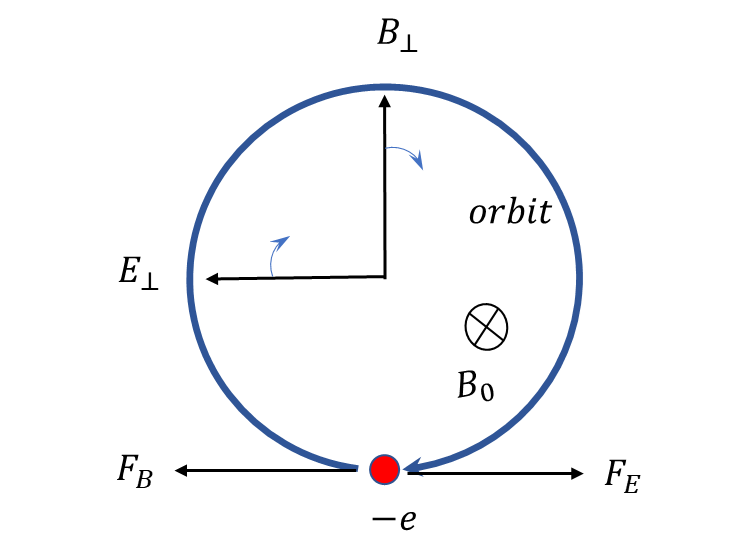
\includegraphics[width=12cm]{image80.png}
\caption{\label{fig:2Dorbite}相对电子平行运动静止坐标系中垂直方向电子受力分
析,其中$F_B$表示电磁波磁场洛伦兹力,$F_E$表示电磁波电场力,$E_\perp$表示电磁波电场,$B_\perp$表示电磁波磁场,$B_0$表示背景磁场}
\end{figure}
这里取相对静止坐标系为研究对象,对电子-电磁波共振时受力分析。如\autoref{fig:2Dorbite}所示,为简单起见,这里只考虑电磁波平行于背景磁场z方向,忽略背景电场。垂直方向电子受电磁波的力分别为
\begin{equation}
\begin{aligned}
\boldsymbol{F}_{\boldsymbol{B} \perp} & = (-e) \boldsymbol{v}_{\|} \times 
\boldsymbol{B}_{\perp}  = \frac{e v_{\|} k}{w} \boldsymbol{E}_{\perp} = \frac{e v_{\|} }{c'} \boldsymbol{E}_{\perp}\\
\boldsymbol{F}_{\boldsymbol{E \perp}} & = (-e) \boldsymbol{E}_{\perp}
\end{aligned}\label{eq:Fperp}
\end{equation}
其中利用到$\vB_⊥=(\vk×\vE_⊥)/ω$,$c'=ω/k$,$k=k_z$。电子在这些力的作用下会通过调节相位使其
运动方向平行于受力方向。垂直方向合力为
\begin{equation}
\vF_{\perp}=\vF_{B \perp}+\vF_{E \perp}=e \vE_{\perp}\left(\frac{v_{z}}
{c^{\prime}}-1\right)=\vF_{E \perp}\left(1-\frac{v_{z}}
{c^{\prime}}\right)
\end{equation}
平行于z轴方向上
电子受电磁波的力为:
\begin{equation}
\boldsymbol{F}_{\|}=-e\left(\boldsymbol{v}_{\perp} \times \boldsymbol{B}_{\perp}
\right)=\frac{-e \boldsymbol{v}_{\perp} \cdot \boldsymbol{E}_{\perp}}{c'}=
\frac{\vv_\perp\cdot \vF_{E\perp}}{c'}
\end{equation}
电磁波对电子做的总功率为
\begin{equation}
P=\vF_\parallel \cdot\vv_\parallel+\vF_\perp \cdot\vv_\perp=\vF_{E\perp}\cdot \vv_\perp
\end{equation}
\noindent 根据以上方程,我们可以得到如下结论:
\begin{enumerate}
\item
对于多普勒效应,$v_z/c' <1$。当$\vF_{⊥}∙\vv_⊥>0$时,有$\vF_{E⊥}∙\vv_⊥>0$,$\vF_\parallel>0$,电磁波加
热电子回旋运动并
对电子存在沿z轴方向的推动力。当$\vF_{⊥}∙\vv_⊥<0$时,有$\vF_{E⊥}∙\vv_⊥<0$,$\vF_\parallel<0$,电子损失动能和回旋内能。对于存在外界电磁波的系统,根据\autoref{eq:Fperp},由于
$abs(\vF_{E⊥})>abs(\vF_{B⊥})$,电子垂直方向速度更倾向于平行于$\vF_{E⊥}$,因此$\vF_{⊥}∙v_⊥>0$,$\vF_{E⊥}∙\vv_⊥>0$,$\vF_\parallel<0$,$P>0$,此时电子吸收电磁波动能增加和回旋内能。
\item
对于切伦科夫效应,$v_z/c' =1$,$\vF_⊥=0$,因此$<F_∥> 
=0$, 
$\vF_⊥∙\vv_⊥=0$,<>表示对时间平均,因此切伦科夫共振时电磁
波对电子的影响
可以忽略,这一点在模拟上也可以看出,切伦科夫共振时电子
速度没有发生剧烈
变化。切伦科夫共振主要是通过静电波和电子相互作用。这时
电子速度和静电波
相速度相同,在电子坐标系中电子看到稳定的电场,在等离子体
体中这种现象也称为朗道共振。
\item
对于反常多普勒效应,$v_z/c' >1$。当$\vF_{⊥}∙v_⊥>0$时,有$\vF_{E⊥}∙v_⊥<0$,$\vF_\parallel<0$,电磁波在垂直方向对
电子做正功,在平
行方向做负功。当$\vF_{⊥}∙\vv_⊥<0$时,有$\vF_{E⊥}∙\vv_⊥>0$,$\vF_\parallel>0$,电磁波在垂直方向对
电子做负功,在平
行方向做正功。对于存在外界电磁波的系统,根据\autoref{eq:Fperp},由于
$abs(\vF_{E⊥})<abs(\vF_{B⊥})$,电子垂直方向速度更倾向于平行于$\vF_{B⊥}$,因此$\vF_{⊥}∙v_⊥>0$,$\vF_{E⊥}∙\vv_⊥<0$,$\vF_\parallel<0$,$P<0$,此时电子释放电磁波同时减小动能并增加回旋内能。

\end{enumerate}\par
在以上过程中
电磁波的磁场分量起到了重要作用,它的性能就像一座连接平行方向和垂直方向的
桥梁,实现能量从动
能输送到旋转内能双向输运。这一基本物理过程有助于理解为什么平行
动能可以转化为旋
转能量。至此,我们通过经典电动力学的角度分析了三种共振状态下电
子的运动特征。根
据以上分析,ADE会导致电子通过散射平行方向动量阻碍平行方向动量增加,那
么如果增加电磁波的能量会对电子运动造成什么影响?
\subsection{ADE对电子的约束}
为了进一步研究 电磁波能量通过$ \mathrm{ADE}  $对电子运动的影响, 我们取左旋电磁波为研究对象, 电磁波参数和背景环境设置分别为  $
\theta=0$, $ \mathbf{k}=10^{5} / \mathrm{m}$, $\quad \mathbf{B}_{0}=200 
\mathrm{Gs}$,$ \omega=1.5 \omega_{\mathrm{c} 0}, \mathbf{E}_{0}=-2.5 
\mathrm{V}  $。电磁波中电场强度$ \mathbf{E}_{\mathbf{w}}  $与静电场强度  
$E_{0}$之比分别为$E_{\mathrm{w}} / E_{0}=1,2,4,6,8 $ 。计算结果如\autoref{fig:findE} 所示, 从图中可以看出, 当 $ E_{\mathrm{w}} / E_{0}>2$ , 在电
子速度达到共振条件时, 电子平行方向速度不再增加, 此时电 子垂直速度迅速增
加, 电子平行方向速度被电磁波约束。
\par 为了研究不同电磁波参 数下阈值大小, 我们
取不同的  $\mathbf{k}, \mathbf{E}, \mathbf{B}_{0}, \omega, \mathbf{E}_{0}$ , 以
无量纲参数  $\frac{\omega^{2}}{k c  \omega_{c 0}} $ 为自变量得 到临界电
场阈值$  E_{c} $ 和背景加速电场  $E_{0}  $比值关系。 这里取电磁波传播方向$\vec k$与背景磁场夹角$\theta_k$分别为$\theta_k=0^o,15^o,30^o$。如\autoref{fig:numEc}所示,当电子被 平行磁场传播的左旋电磁波约束时, 电磁波的电场阈值约为背景
电场的 3 倍 。当电磁波传播方向与背景磁场夹角增大时,临界阈值有下降的趋势,造成这种现象有可能是因为电磁波电场分量在$B_0$方向增加,导致平行方向阻尼增加,具体原因有待进一步研究。
\begin{figure}
\centering
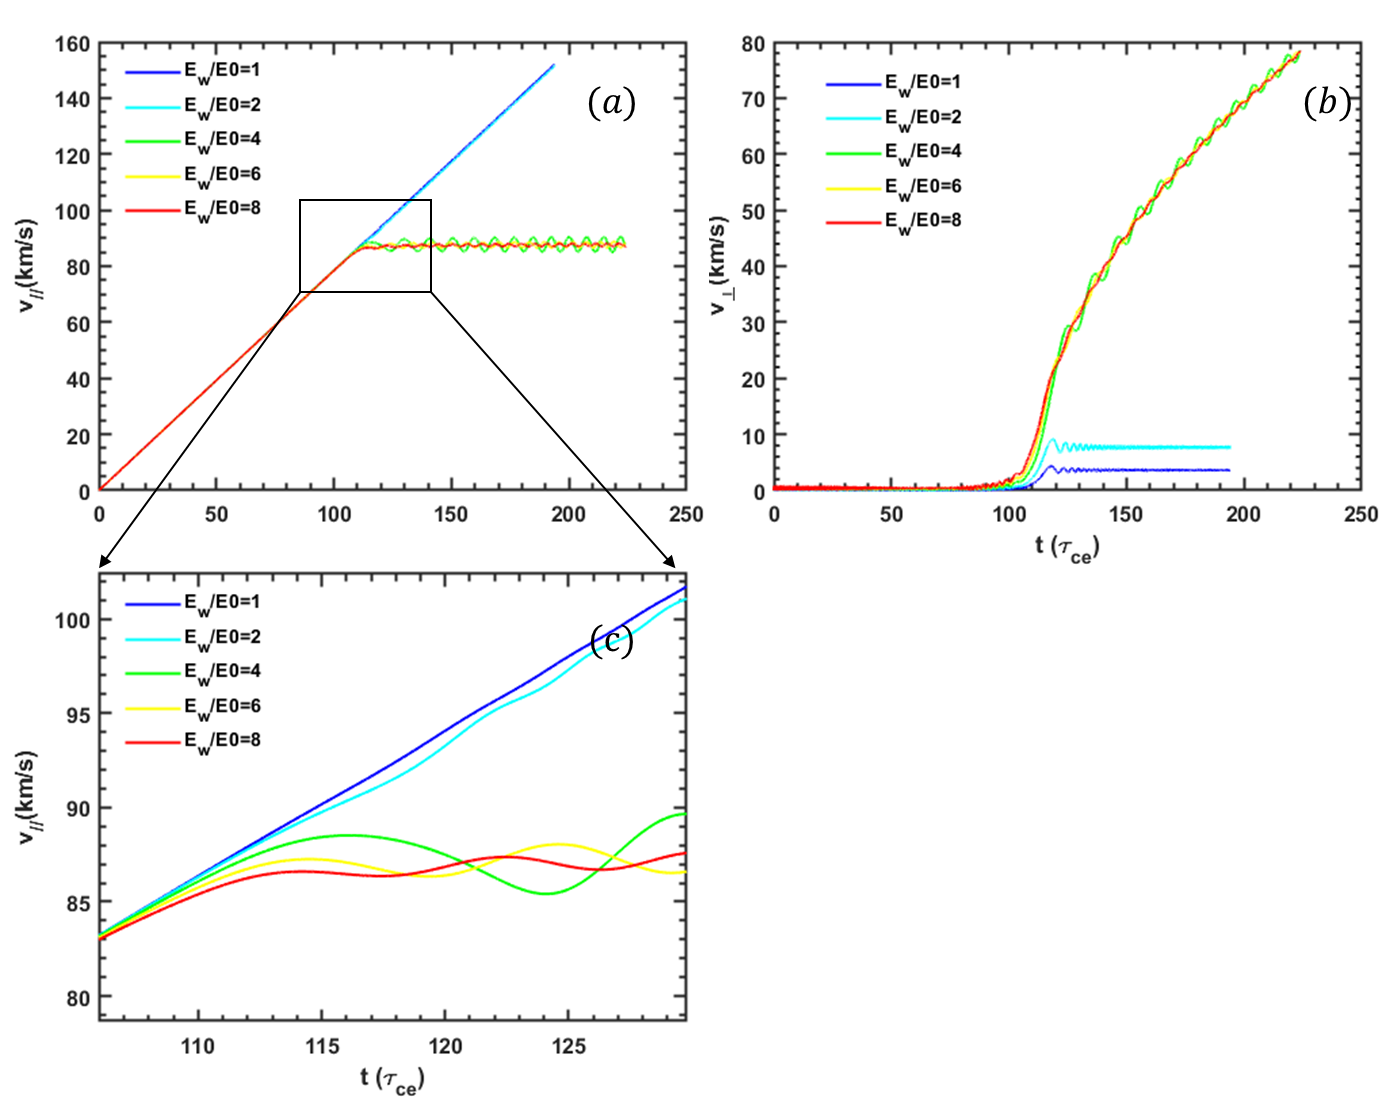
\includegraphics[width=11cm]{image81_1.png}
\caption{\label{fig:findE}不同电磁波能量下电子速度演化。(a)平行方向速度演化图(b)垂直方向速度演化图(c)平行方向速度演化图的局部放大}
\end{figure}

\begin{figure}
\centering
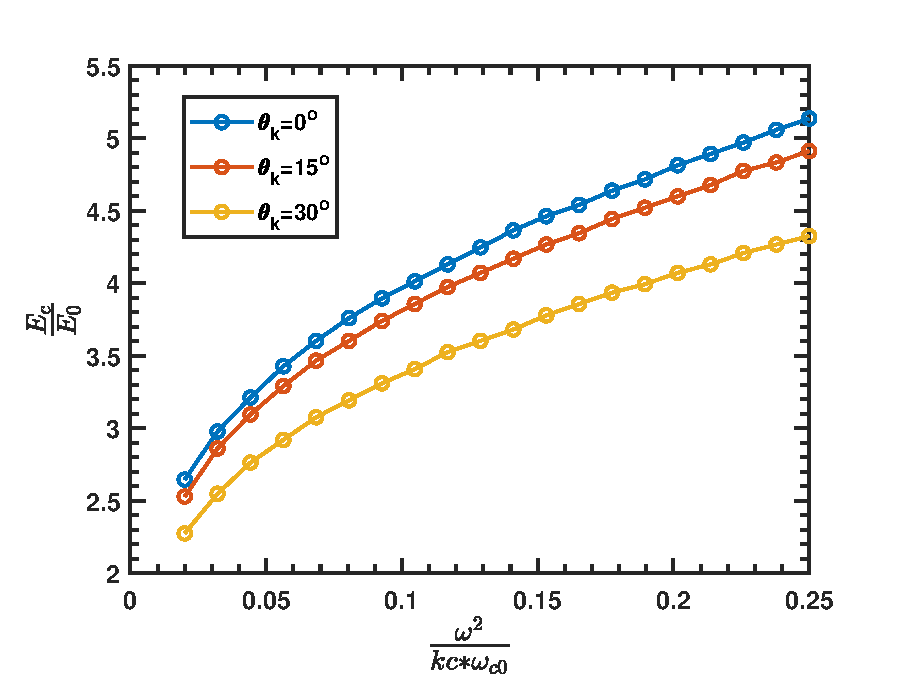
\includegraphics[width=11cm]{image82.eps}
\caption{\label{fig:numEc}约化阈值电场与无量纲化参数$ω^2/(kcω_{c0} )$变化关系}
\end{figure}
%\clearpage
\subsection{量子与电动力学描述的等效性}
一般经典力学适用于宏观物理,而量子力学多用于解释微观物理过程。这里用两种不同的方法解释同一个物理现象,究竟是否等价还需要经过检验。
从量子角度上考虑磁化电子和电磁波相互作用,其能量方程为(可参考\autoref{sec:quantum}):
\begin{equation}
\Delta T_{12}=\hbar\omega+\Delta U_{21}
\end{equation}
在满足反常多普勒共振条件下时, 当磁化电子发射能量为  $\hbar \omega $ 的电磁波时, 电子损失的动量为  $\Delta T_{12}=\hbar k v \cos \theta $, 电子增加的内能为  $\Delta U_{21}=\hbar \omega_{c e}$。因此电子动能 转化为内能的比率为 $ \eta_{p}=\frac{\hbar \omega_{c e}}{\hbar k v \cos \theta}=\frac{\omega_{c e}}{k v \cos \theta}$ , 动能转化为电磁波的比率为$  \eta_{\omega}=\frac{\omega}{k v\cos \theta} $。 根据电动力学基本物理法则, 我们可以准确地计算出当共振发生时电子动能损失 量、激发的电磁波能量以及电子回旋内能的增加量 (这里指电子回旋动能), 然后依此对比经典电动力学得到的电子能量转化率和量子得到的转化率,验证两种方法得到的结果是否一致。

模拟参数分别为$θ=0$,$k=10^5~/m$, $B_0=200~Gs$,$ω=1.5ω_{c0}$,$E_0=-2.5~V$,左旋偏振波,电磁波电场振幅$E_p=19~V/m$,电子初始速度为0,初始空间位置为[0   , 0   ,  0]。计算结果如\autoref{fig:traporbit} 所示,当电子速度满足反常多普勒共振条件时,电子共振约束,垂直方向能量不断增加,导致轨道结构出现喇叭结构,同时平行方向速度不再受电场加速,电场驱动能部分转化为垂直方向回旋内能,导致动量相空间出现扁平圆盘结构。 \autoref{fig:vtevo}展示了该模拟参
\begin{figure}
\centering
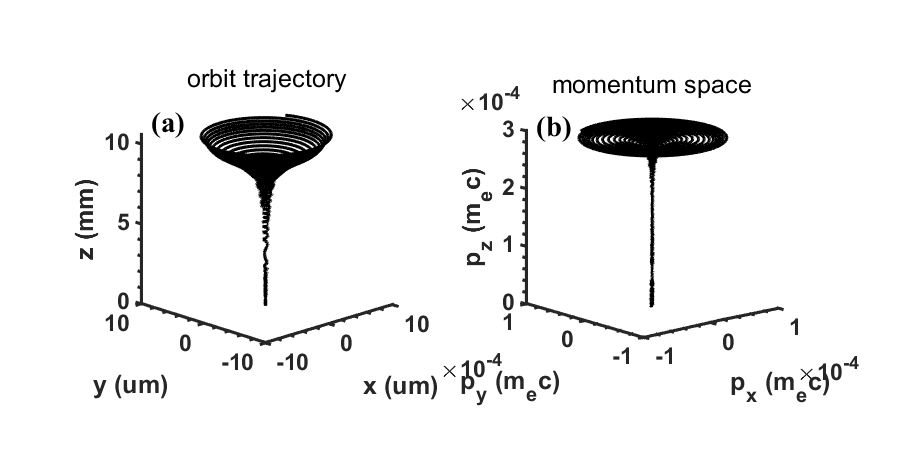
\includegraphics[width=12cm]{traporbit.eps}
\caption{\label{fig:traporbit}(a)电子运动轨道图(b)电子动量相空间图}
\end{figure}
数下电子各参数的演化过程,分别为(a)电子垂直速度演化(b)电子平行速度演化和(c)电子共振频率演化。根据电子共振时平行速度可以计算出单位时间内静电场对电子做功功率为$-eE_0 v_c$。通过对电子做功分析我们可以进一步研究能量转移机制,如   \autoref{fig:Wpevo}所示。

电磁波平行方向和垂直方向对电子做功以及电磁波对电子做的总功如\autoref{fig:Wpevo}(a)所示。当ADE共振发生时,平行磁场方向电磁波对电子做负功,垂直磁场方向电磁波对电子做正功,二者之和为负,说明共振过程电磁波对电子做的总功为负,共振过程电磁波会吸收电子的能量,导致电磁波能量变大;
将平行磁场方向做功分解为静电场做功和电磁波磁场洛伦兹力(由于电磁波传播方向平行与背景磁场,此时平行磁场方向电磁波只存在洛伦兹力)做功得\autoref{fig:Wpevo}(b),当共振发生时平行方向电磁波做负功,静电场始终做正功,静电场做功和电磁波洛伦兹力做功功之和正好等于电子平行方向动能$T_{k∥}$,满足能量守恒定律。由此我们得到结论:反常多普勒共振时电磁波磁场分量会转移平行方向静电场功;
将垂直方向做功分解为电磁波电场做功和磁场做功得到\autoref{fig:Wpevo}(c)。垂直方向电磁波磁场做功$W_{B⊥}$为正,电磁波电场做功$W_{E⊥}$为负,电磁波做的总功$W_{⊥emw}$等于电子垂直方向动能$T_{k⊥}$(这里就相当于电子的回旋内能),满足能量守恒定律。因此得到结论:共振过程中被磁场散射的平行方向静电场功转化为电子的回旋内能和电磁波。电磁波磁场本身不做功,只是功的搬运工,将静电场能量输运到电子回旋内能以及电磁波。以上所有结果和\autoref{sec:force}分析定性一致;
电子静电功能量转移率如\autoref{fig:Wpevo}(d)所示。通过计算共振过程中平行方向静电场做功功率 以及垂直方向电子回旋内能增加速率和电磁波增加速率, 我们可以得到静电场能 量转移至回旋内能比率 $ \eta_{p}$  以及电磁波比率$  \eta_{\omega}$ 。根据计算结果可以看出 $ \eta_{p} \approx 0.39 $, $ \eta_{\omega} \approx 0.61 $ 。从量子力学上, 转移效率率应为$  \eta_{p}=\frac{\omega_{c e}}{k v \cos \theta}$, $\eta_{\omega}=\frac{\omega}{k v\cos \theta}$, 将参数 $ \omega_{c e}=   3.52 \times 10^{9} ~ \mathrm{s^{-1}}$, $\mathrm{k}=10^{5} ~ \mathrm{m^{-1}}, \theta=0, \mathrm{v}=8.7 \times 10^{4}  ~\mathrm{m^{-1}}$, $\omega=5.28 \times 10^{9} ~\mathrm{s^{-1}} $代入得到  $\eta_{p} \approx 0.40$, $\eta_{\omega} \approx  0.60 $, 二者结果基本一致。由此可见关于  $\mathrm{ADE}  $量子力学和电动力学的描述具有 等效性。
\clearpage
\begin{figure}
\centering
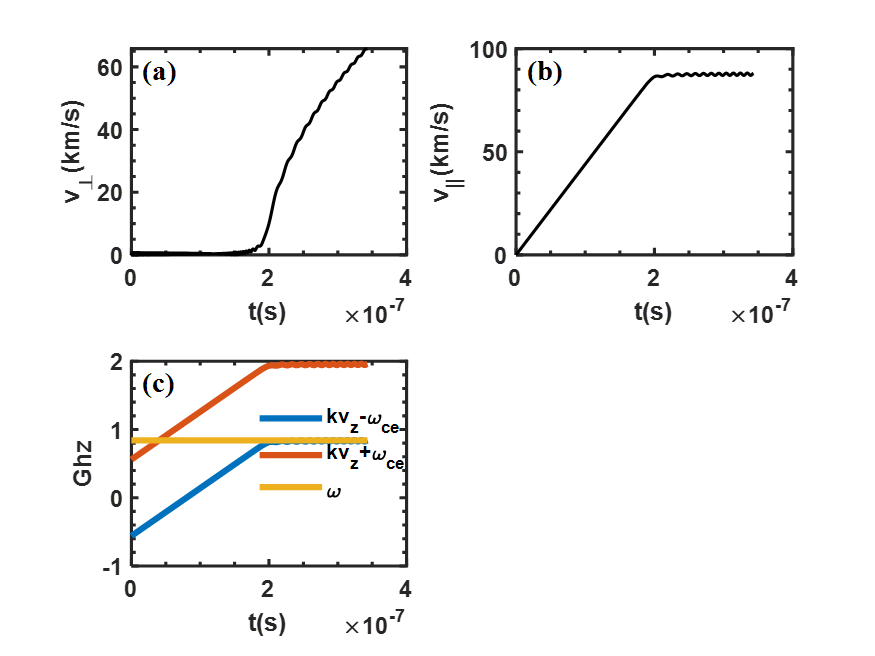
\includegraphics[width=11cm]{image84.png}
\caption{\label{fig:vtevo}(a)电子垂直速度演化(b)电子平行速度演化(c)电子共振频率演化}
\end{figure}
\begin{figure}
\centering
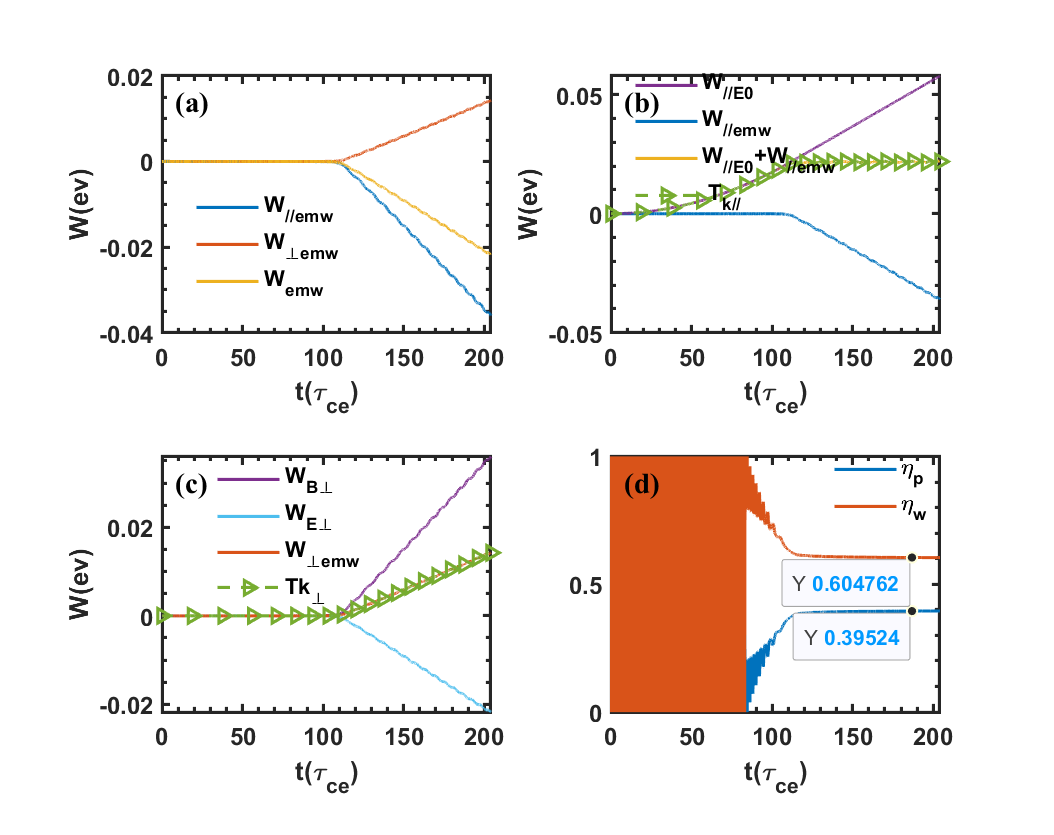
\includegraphics[width=11cm]{image85.eps}
\caption{\label{fig:Wpevo}a)电磁波对电子做功分析(b)平行方向静电场和电磁波对电子做功(c)垂直方向电磁波对电子做功(d)静电功能量转化比率,
其中$\eta_p$表示静电场能量转移至回旋内能比率,$\eta_\omega$表示静电场能量转移到电磁波比率.}
\end{figure}
\clearpage
\subsection{托卡马克参数下电子ADE的超算模拟}\label{sec:tokamakade}
托卡马克参数一般满足  $\mathrm{B}_{0}=2 ~\mathrm{T}$, 对应电子回旋频率约为 $ 56 ~\mathrm{Ghz} $。 根据计算对 步长的要求$  \Delta t=\min \left(\frac{2 \pi}{50(k \cdot v)}, \frac{2 \pi}{50 \omega}, \frac{2 \pi}{50 \omega_{c 0}}\right)$ , 单位步长至少不能超过 $ 3.6 \times 10^{-13} ~\mathrm{s^{-1}} $。为了简化计算条件, 同样以均匀背景空间为计 算环境,考虑 马克中环电场强度为$  E_{0}=-0.2 ~\mathrm{V} $,  取上杂化附近电磁波参数, 频率为  $\omega=\omega_{c e}, k=2.6 \times 10^{3} / \mathrm{m} $ (为什么选 这个参数会在后文给出)。 当 $ \theta=0$ , 根据 $ \omega=\boldsymbol{k} \cdot \boldsymbol{v}-\omega_{c e} $ 得电子共振速度约为$  v_{c}=2.26 \times 10^{8} ~\mathrm{m} / \mathrm{s}$ , 对应的电子动能为$  0.26 ~\mathrm{MeV} $ 。电子速度从 0 加速到  $v_{c}$  约需要$  0.01 ~\mathrm{s}$ , 至少要计算 $ 2.8 \times 10^{10} $ 步, 个人计算机无法具备如此巨大的数据处理能力, 只有超级计算机才能处理该过程。 同时模拟长时间尺度物理过程容易造成数值误 差累积, 这也是采用保体积算法的理由。\par
  这里通过山河超算计算了托卡马克参数下电子反常多普勒共振过程。模拟参数设置为:$B_0=2~T, E_0=-0.2~V, k=2.6×10^3~m^{-1}$, 左旋偏振波,电磁波电场振幅$E_p=40~V/m$(对应的能流约为$S\approx 9~W/m^2$),电子初始速度为0,初始空间位置为[0, 0 ,0]。\autoref{fig:Tokaevo}展示了 k与B夹角从$θ=0^o-75^o$区间电子运动状态演化图,当电子速度加速到满足ADE条件时,电子平行方向速度不再增加,垂直方向迅速上升。图中黄色虚线为不同电磁波入射角下电子初始满足ADE共振条件所对应的时间和角度关系,即$ω+ω_{ce} (t)-k∙v(t)=0$,夹角越大达到共振所需要的平行速度越高,
因此共振时间越晚。共振发生后,电子将受到电磁波作用不断将静电场能量转移到垂直方向,并始终保持共振条件。这验证了托卡马克参数下ADE约束能力同样适用。

\begin{figure}
\centering
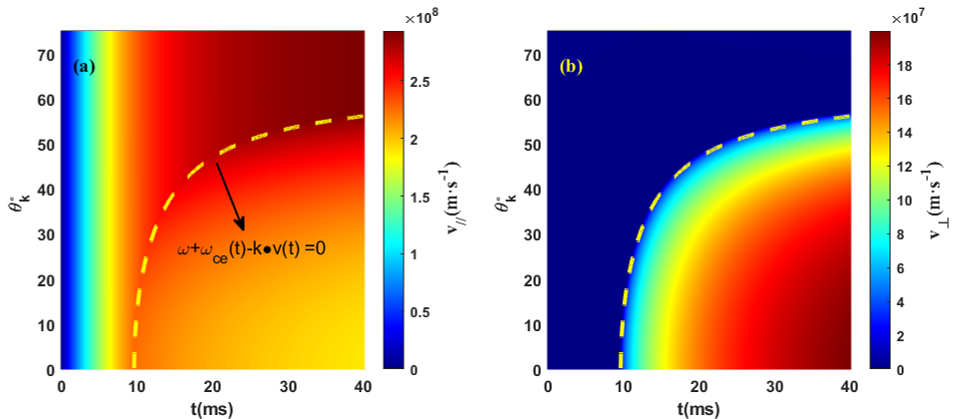
\includegraphics[width=14cm]{image86.png}
\caption{\label{fig:Tokaevo}不同电磁波入射角下电子速度演化图,其中(a)电子平行速度随时间演化(b)电子垂直速度随时间演化}
\end{figure}

\subsection{抑制逃逸电子的新方法}
\par \noindent
1.抑制逃逸电子常用方法

高能逃逸电子通常会在破裂或高参数放电过程中产生,如果不加控制高达几十Mev的逃逸电子会对托卡马克装置内壁造成严重破坏,影响内部硬件的使用寿命。目前托卡马克系统中采取了各种方法抑制逃逸电子的破坏力,最常见的有:
\begin{enumerate}
\item [(a)]
注入工作气体。通过提高等离子体密度增加逃逸电子临界电场,抑制逃逸电子产生\cite{RN954}。
\item[(b)]
	注入杂质气体。逃逸电子通过和高Z的杂质气体 (Ar,Ne)的束缚电子、或离子碰撞散射,导致逃逸电子能量耗散,杂质气体起到了快速抑制逃逸电子能量的作用,减小逃逸电子产生速率\cite{RN2118}。
\item[(c)]
	增加边界磁扰动。增加磁扰动可以降低逃逸电子约束时间使得逃逸电子在形成你高能逃逸电子之前就已经损失\cite{RN1485}。
\end{enumerate}
除此之外,还有通过注入MW量级的低杂波等方式来降低逃逸电子密度\cite{RN1866},低杂波和高能逃逸电子通过反常多普勒共振的作用抑制逃逸电子增长,但是同时又会通过朗道共振的机制产生大量非热电子,当低杂波关闭时会带来更多的高能逃逸电子,这是这种方式的弊端。常用的方式都会改变了等离子体运行状态,使得放电过程无法保持稳定。其中注入杂质气体还需要依赖于大数据根据诊断信号的变化提前预测破裂发生的时间,及早将杂质气体注入才能避免高能逃逸电子的产生,这对数据分析模型又提出很高的要求,同时注入的杂质气体还会降低下一炮的放电品质。面对这些问题,如果能找到更加干净、稳定的方法实现抑制逃逸电子,对保护托卡马克装置和提高放电品质都有一定的积极意义。
\par \noindent
2.托卡马克中高能电子与波的激发


在行波管结构中(如\autoref{fig:TEO}所示)慢波管道内壁周期性结构(如\autoref{fig:slowstru}(a))产生了类似\autoref{fig:slowstru}(b)结构的本征电磁模\cite{RN2120}。由电子枪产生的束电子经过加速穿过行波管道时,相速度和电子运动速度相同的波会和电子通过朗道共振激发电磁波,实现将电子能量传递给电磁波。
\begin{figure}
\centering
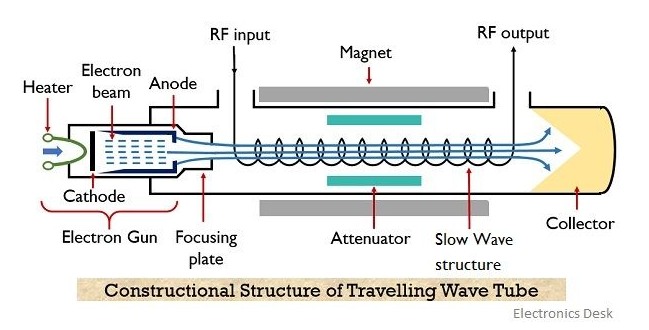
\includegraphics[width=14cm]{image87.png}
\caption{\label{fig:TEO}\href{https://electronicsdesk.com/travelling-wave-tube.html}{行波管结构图}	}
\end{figure}
\begin{figure}
\centering
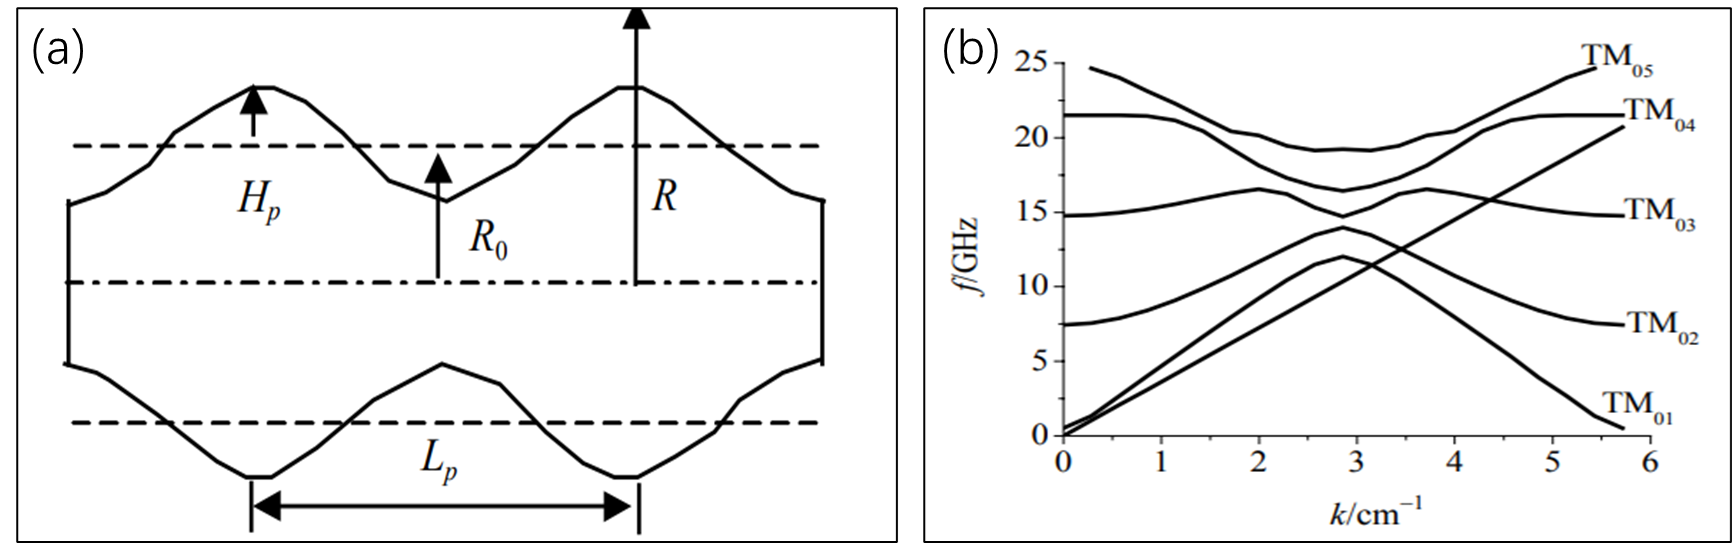
\includegraphics[width=14cm]{image88.png}
\caption{\label{fig:slowstru}(a) 慢波结构内壁(b)慢波结构本征电磁模与电子束朗道共振频率[158]	}
\end{figure}

同理在托卡马克装置中,磁化等离子体中存在的本征电磁模也会和高能电子相互作用。高能电子和电磁波之间的共振机制通常可分为多普勒共振、朗道共振和反常多普勒共振,这三种共振机制共同作用在等离子体本征模上导致波的阻尼或增长,而激发出的电磁波又会改变电子的运动状态。那么能否利用磁化等离子体中本征波通过ADE抑制逃逸电子?首先问题是哪些波可以产生ADE效应,其次是这种波能否被激发出来。为了回答这些问题,首先分析磁化等离子体存在哪些类型电磁波。

为了方便,以冷等离子体条件为出发点,冷等离子体色散关系由如下方程给出\cite{RN1595}:
\begin{equation}\label{eq:dispw}
%\begin{aligned}
% \omega^{10} -&\omega^{8}\left(2 k^{2} c^{2}+\omega_{c e}^{2}+\omega_{c i}^{2}+3 \omega_{p}^{2}\right) \\
%+&\omega^{6}\left[k^{4} c^{4}+\left(2 k^{2} c^{2}+\omega_{p}^{2}\right)\left(\omega_{c e}^{2}+\omega_{c i}^{2}+2 \omega_{p}^{2}\right)+\left(\omega_{p}^{2}+\omega_{c e} \omega_{c i}\right)^{2}\right] \\
%-&\omega^{4}\left[k^{4} c^{4}\left(\omega_{c e}^{2}+\omega_{c i}^{2}+\omega_{p}^{2}\right)+2 k^{2} c^{2}\left(\omega_{p}^{2}+\omega_{c e} \omega_{c i}\right)^{2}\right. \\
%+&\left.k^{2} c^{2} \omega_{p}^{2}\left(\omega_{c e}^{2}+\omega_{c i}^{2}-\omega_{c e} \omega_{c i}\right)\left(1+\cos ^{2} \theta\right)+\omega_{p}^{2}\left(\omega_{p}^{2}+\omega_{c e} \omega_{c i}\right)^{2}\right] \\
%+&\omega^{2}\left\{k^{4} c^{4}\left[\omega_{p}^{2}\left(\omega_{c e}^{2}+\omega_{c i}^{2}-\omega_{c e} \omega_{c i}\right) \cos ^{2} \theta+\omega_{c e} \omega_{c i}\left(\omega_{p}^{2}+\omega_{c e} \omega_{c i}\right)\right]\right. \\+&\left.k^{2} c^{2} \omega_{p}^{2} \omega_{c e} \omega_{c i}\left(\omega_{p}^{2}+\omega_{c e} \omega_{c i}\right)\left(1+\cos ^{2} \theta\right)\right\} \\
%-&k^{4} c^{4} \omega_{c e}^{2} \omega_{c i}^{2} \omega_{p}^{2} \cos ^{2} \theta 
%= 0
%\end{aligned}
\begin{aligned}
\omega^{10} & -\omega^{8}\left(2 k^{2} c^{2}+\omega_{c e}^{2}+\omega_{c i}^{2}+3 \omega_{p}^{2}\right) \\& +\omega^{6}\left[k^{4} c^{4}+\left(2 k^{2} c^{2}+\omega_{p}^{2}\right)\left(\omega_{c e}^{2}+\omega_{c i}^{2}+2 \omega_{p}^{2}\right)+\left(\omega_{p}^{2}+\omega_{c e} \omega_{c i}\right)^{2}\right] \\& -\omega^{4}\left[k^{4} c^{4}\left(\omega_{c e}^{2}+\omega_{c i}^{2}+\omega_{p}^{2}\right)+2 k^{2} c^{2}\left(\omega_{p}^{2}+\omega_{c e} \omega_{c i}\right)^{2}\right. \\& \left.+k^{2} c^{2} \omega_{p}^{2}\left(\omega_{c e}^{2}+\omega_{c i}^{2}-\omega_{c e} \omega_{c i}\right)\left(1+\cos ^{2} \theta\right)+\omega_{p}^{2}\left(\omega_{p}^{2}+\omega_{c e} \omega_{c i}\right)^{2}\right] \\& +\omega^{2}\left\{k^{4} c^{4}\left[\omega_{p}^{2}\left(\omega_{c e}^{2}+\omega_{c i}^{2}-\omega_{c e} \omega_{c i}\right) \cos ^{2} \theta+\omega_{c e} \omega_{c i}\left(\omega_{p}^{2}+\omega_{c e} \omega_{c i}\right)\right]\right. \\& \left.+k^{2} c^{2} \omega_{p}^{2} \omega_{c e} \omega_{c i}\left(\omega_{p}^{2}+\omega_{c e} \omega_{c i}\right)\left(1+\cos ^{2} \theta\right)\right\} \\& -k^{4} c^{4} \omega_{c e}^{2} \omega_{c i}^{2} \omega_{p}^{2} \cos ^{2} \theta  = 0
\end{aligned}
\end{equation}
其中$ω_p$为等离子体频率,$ω_{ce}$为电子回旋频率,$ω_{ci}$为离子回旋频率,θ表示波矢与B的夹角。根据\autoref{eq:dispw},$ω_p/ω_{ce}$ =0.5条件下不同角度等离子体色散关系如\autoref{fig:Disper}所示,图中蓝色表示$θ=0$对应的色散曲线,红色表示$90^o$对应的色散关系,X表示垂直磁场传播的非寻常波,O表示垂直磁场传播的寻常波,R表示平行磁场传播的右旋波,L表示平行磁场传播的左旋波。根据ADE共振条件,只有相速度低于光速的波才能有可能参与反常多普勒共振,因此整个色散关系图中只有A、B区域的波可以产生ADE效应。由于左旋波是导致电子产生反常多普勒效应的主要机制,实际上对于任何波只要不是纯右旋偏振都可以分解出左旋分量,但相对分量大小与波的主要偏差态有关。等离子体中电磁波的偏振态可如下表示\cite{RN1452}
\begin{equation}
\vE=A\left(e_{x}+i e_{y}+e_{z}\right) e^{i(k \cdot r-\omega t)}
\end{equation}
其中
\begin{align}
e_{x}   =& 1 \\
e_{y}  = & \frac{\frac{\omega_{p e}^{2} \omega_{c e}}{\omega}}{\omega^{2}-k^{2} c^{2}-\omega_{c e}^{2}-\omega_{p e}^{2}+\frac{k^{2} c^{2} \omega_{c e}^{2}}{\omega^{2}}} \\
e_{z}  = &\frac{k_{\|} k_{\perp} c^{2}}{\omega_{p e}^{2}+k_{\perp}^{2} c^{2}-\omega^{2}}
\end{align}
$e_y$大于零表示波主要具有右旋特征,反之具有左旋特征(这里$\omega_{c e}>0$,故$e_{y}$ 、$ e_z$与参考文献中对应的公式相差一个负号) 。在\autoref{fig:Disper}中虚线之间$e_y$小于零,虚线之外$e_y$大于零,因此A区间的波更具有产生ADE效应的潜能。当然B区间也可以发生反常多普勒效应,如最近讨论较多的哨声波激发\cite{RN975,RN1815},只是原则上A区间的激发条件要低于B区间, G.I.Pokol也曾通过计算波的阻尼率论证过这点\cite{RN1757}。\par
考虑电子和波共振能量,逃逸电子和波若产生共振必须要满足共振条件
\begin{equation}\label{eq:resonants}
\omega+n \omega_{c e}-\boldsymbol{k} \cdot \boldsymbol{v}=0
\end{equation}
将\autoref{eq:resonants}和\autoref{eq:dispw}结合我们可得到共振动量与频率角度$\theta$的关系,这里取速度v完全
\begin{figure}[ht]
\centering
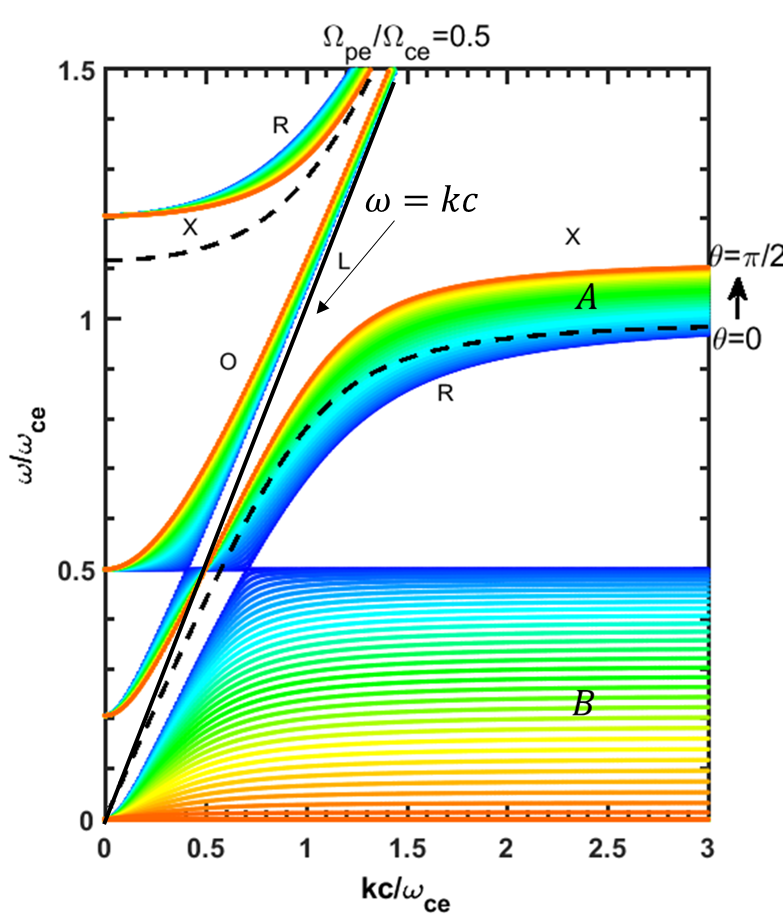
\includegraphics[width=12cm]{image90.png}
\caption{\label{fig:Disper}冷等离子体色散关系图}
\end{figure}
平行于磁场,n=1为反常多普勒共振。如\autoref{fig:Pcontou},对于A区间,ADE共振约化动量大于1的共振曲线都经过\autoref{fig:Pcontou}(c)中右下角区间。该区间对应频率主要在上杂化共振层附近$\omega \sim\left(\omega_{c e}, \sqrt{\omega_{c e}^{2}+\omega_{p}^{2}}\right)$,这说明了为什么磁化装置中发生电子角度快速散射时会激发出上杂化共振层附近频率的电磁波\cite{RN786,RN1868}。另一方面A区间的朗道共振约化动量同样几乎都大于1(\autoref{fig:Pcontou}(a)),这意味着背景热电子对A区间的波的阻尼较小,A区间的波更容易形成。对于B区间,其对应的朗道共振约化动量几乎都小于1(\autoref{fig:Pcontou}(b)),
%\begin{figure}
%\centering
%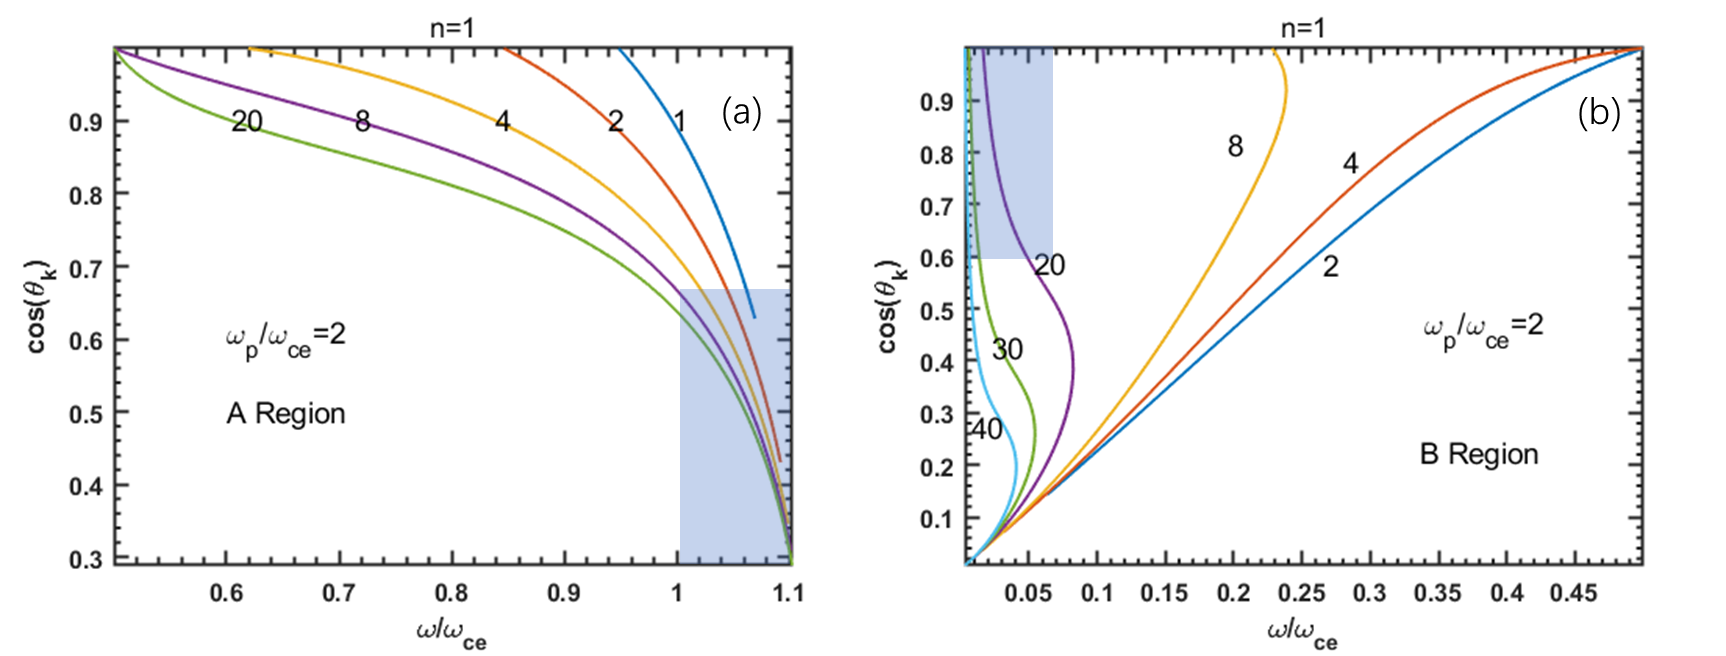
\includegraphics[width=12cm]{image91.png}
%\caption{\label{fig:Pcontou}反常多普勒共振下逃逸电子约化动量与波的共振频率和角度关系(a)A区间,左下边界为不同角度的共振频率,其中$\cos(θ_k)=0$对应上杂化共振频率(b)B区间,右下边界为不同角度共振频率,$\cos(θ_k)=0$对应下杂化共振频率}
%\end{figure}
\begin{figure}[ht]
  \centering
  \begin{overpic}[scale=0.45]{image91_An0.eps}
    \put(25, 55){$(a)$}
  \end{overpic}
  \begin{overpic}[scale=0.45]{image91_Bn0.eps}
    \put(25, 55){$(b)$}
  \end{overpic}  
  \begin{overpic}[scale=0.45]{image91_A.eps}
    \put(25, 55){$(c)$}
  \end{overpic}
  \begin{overpic}[scale=0.45]{image91_B.eps}
    \put(25, 55){$(d)$}
  \end{overpic}  
  \caption{\label{fig:Pcontou}反常多普勒共振下逃逸电子约化动量与波的共振频率和角度关系(a)A区间朗道共振约化动量(b)B区间朗道共振约化动量(c)A区间ADE共振约化动量(d)B区间ADE共振约化动量}%。A区间左下边界为不同角度对应的上杂化共振频率,B区间右下边界为不同角度对应的下杂化共振频率。
\end{figure}
背景热电子对B区间波的朗道阻尼较大,因此需要更多的非热电子成分抵消背景热电子的阻尼才能激发出B区间的电磁波。当高能逃逸电子能量大于10MeV(约化动量p>20)时,高能电子通过ADE效应所激发的电磁波共振曲线几乎会经过\autoref{fig:Pcontou}(d)左上角区间。该区间正好对应接近平行磁场传播的哨声波区域,因此托卡马克实验中当高能电子能量大于10~MeV时通常会伴随哨声波出现\cite{RN786,RN798}。

综上所诉, A区间的电磁波更容易产生反常多普勒共振,而且实验还发现逃逸电子发生反常多普勒共振时会激发出上杂化共振频率附近的非寻常电磁波\cite{RN786,RN1868},但是通过逃逸电子激发的上杂化共振频率附近的非寻常波无法保持稳定存在。逃逸电子通过自身产生的电磁波无法对自身产生稳定持久的散射,因此即使发生了反常多普勒共振,逃逸电子还是不可挽回地继续被加速到更高能量。那么如果反过来通过外界注入电磁波,使其激发上杂化共振层附近电磁波,通过逆向过程原则上也可以实现反常多普勒共振达到抑制逃逸电子的目的。在\autoref{sec:tokamakade}节计算中,约化电磁波频率为1,约化波数$k_n=kc/ω_{ce}=2.2$,正好对应\autoref{fig:Disper}中的A区间坐标 (2.2,1)区域。模拟中电磁波电场$E_p=40~V/m$对应的能流约为$9.5~W/m2$,假设等离子体中电磁极化即使只有1/40的能量可以分解为左旋电磁波,入射电磁波的能流也不过360~W/m2即可实现对逃逸电子稳定的散射约束。因此通过主动注入电磁波至上杂化共振层理论上可以实现对逃逸电子稳定的动量散射,抑制逃逸电子平行能量,同时将平行磁场方向静电场能量转化为垂直磁场回旋“内能”和共振波。此时共振波除了来自外界主动注入的能量还有来自逃逸电子自身通过共振激发出的波,当自身产生的波能量大于耗散时还有可能实现波的放大,进一步达到抑制逃逸电子能量的效果。

\par \noindent
3.冷等离子体中电磁波的传播

通过外界注入非寻常电磁波必须要考虑电磁波在托卡马克装置中传播过程,以便找到合适的注入方法。这里冷等离子体条件为基础,研究波在冷等离子体中的传播过程。冷等离子体折射率为Appleton-Hartree公式
\begin{equation}
n^{2}=1-\frac{X(1-X)}{1-X-\frac{1}{2} Y^{2} \sin ^{2} \theta \pm\left[\left(\frac{1}{2} Y^{2} \sin ^{2} \theta\right)^{2}+(1-X)^{2} Y^{2} \cos ^{2} \theta\right]^{\frac{1}{2}}}
\end{equation}
其中  $X=\frac{\omega_{p e}^{2} }{\omega^{2}}, Y=\frac{\omega_{c e}}{\omega}, \theta=\operatorname{acos}\left(\frac{k \cdot B}{|k \| {B}|}\right)$ ,$\pm$表示两种不同偏振态的电磁波所对应的 折射率。当  $\theta=90^{\circ} $ 时, 即电磁波传播方向垂直于磁场时, +表示  O  波的折射率,-表示X波的折射率。通过自主开发的Ray-Tracing3D程序(可参考附录\autoref{sec:A4})我们可模拟任意角度任意位置发射的电磁波在托卡马克装置等离子体中的传播过程。

考虑托卡马克芯部纵场强度B0=2~T,芯部密度为$n_e=1×10^{19}~m^{-3}$,密度沿径向为
抛物线分布,EAST装置大半经为R0=1.85~m,小半径为a=0.45~m。该背景参数下托卡马克中平面径向方向等离子体特
征频率分布如\autoref{fig:freq}所示。当频率为60GHz入射波从低场侧以相对于X轴夹角为
$20^o$打入等离子体中时,入射波会由于折射率对极化方向的
\begin{figure}
\centering
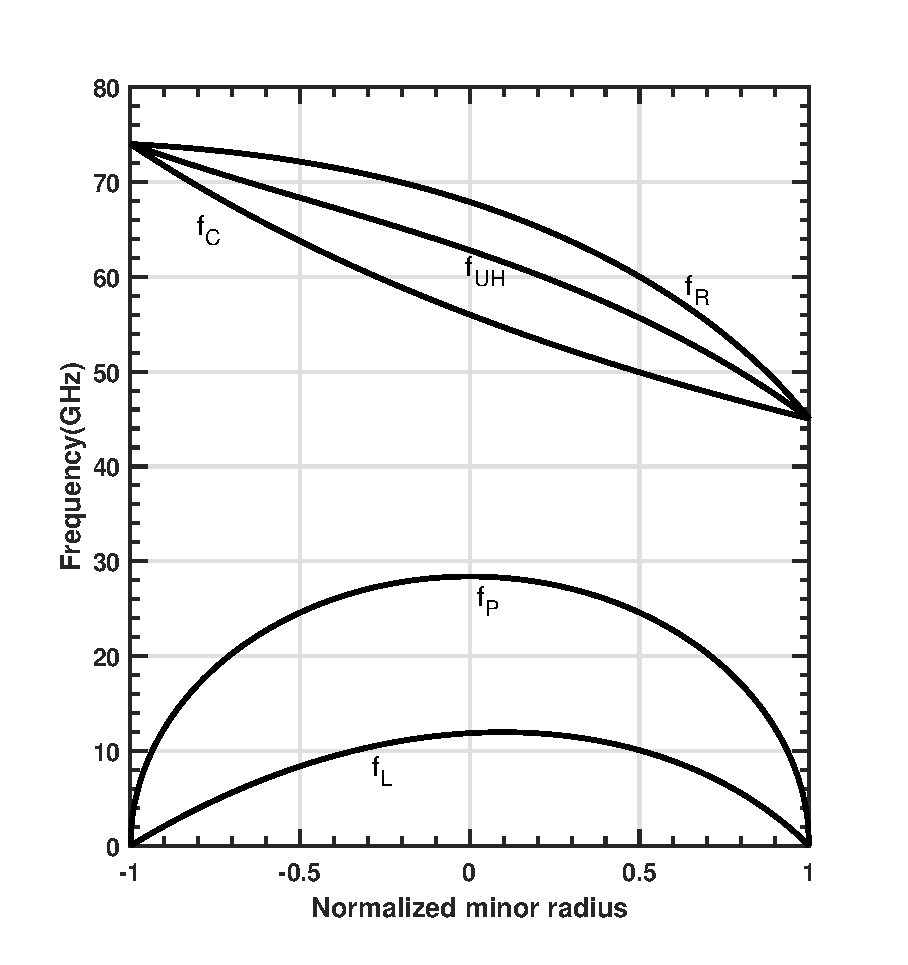
\includegraphics[width=12cm]{image92.eps}
\caption{\label{fig:freq}等离子体中特征频率分布,其中${f_c}$为电子回旋频率,
$f_{UH}$为上杂化频率,$f_{R}$为右旋截止频率,$f_P$为等离子体频率,$f_L$为左旋截止
频率}
\end{figure}
选择出现双折射效应(\autoref{fig:outin}),其中一支对应折射率为n-,具有X波偏振,另一支
为n+,具有O波偏振,其中X波会在右旋截止层附近被反射,而O波直接穿过等离子体。因
此从低场侧注入电磁波无法激发上杂化共振层附近的X波。

如\autoref{fig:inout}(a),当电磁波从高场测以相对X轴85度注入时,其中O波(n2+)会穿过等
离子体,而X波(n2-)分量会在穿过1次电子回旋频率后沉积在上杂化共振层位置形成相速度小于真空光速的X波。其$k_y$波数如\autoref{fig:outin}(b)所示, X波其在上杂化共振层R=1.95~m附近实现$k_y$的增加,使其具备了参与ADE共振的条件,因此在R=1.95~m附近的逃逸电子就有可能会被外界电磁波散射约束。


\begin{figure}[H]
\centering
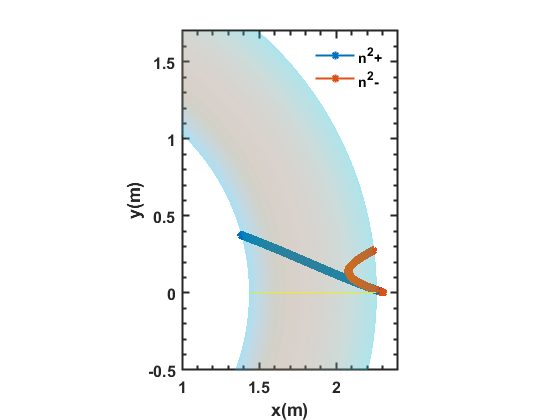
\includegraphics[width=12cm]{image93.png}
\caption{\label{fig:outin}低场侧60GHz电磁波注入}
\end{figure}

\begin{figure}[H]
\centering
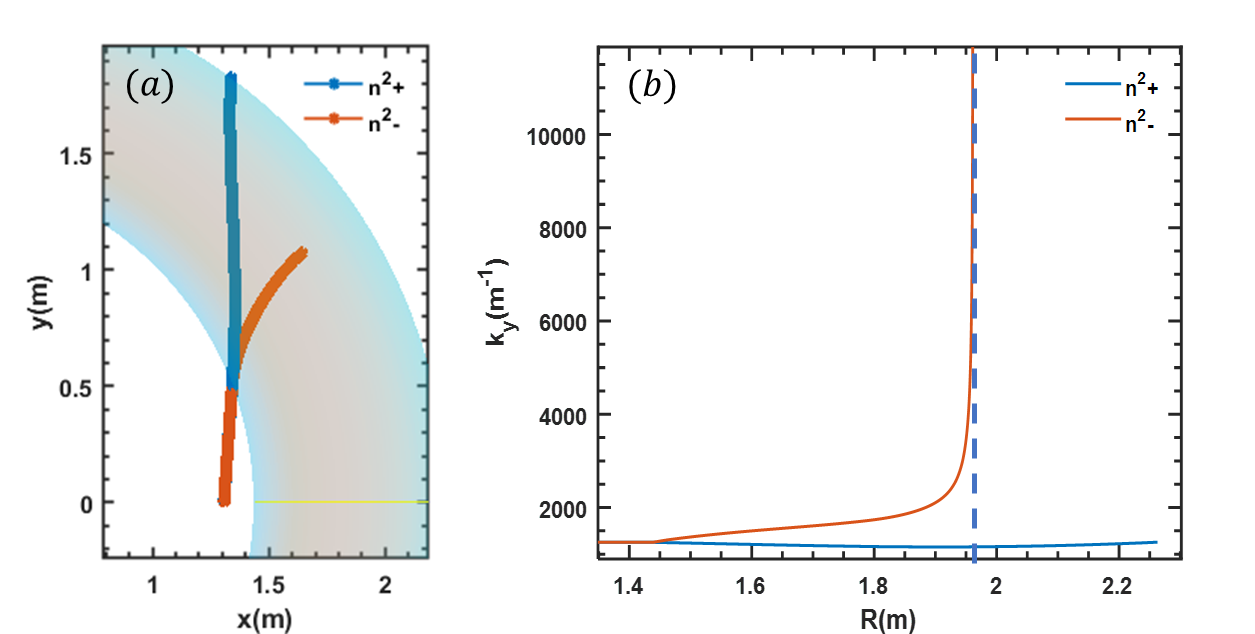
\includegraphics[width=12cm]{image94.png}
\caption{\label{fig:inout}(a) 高场侧60GHz电磁波注入(b)ky波数分布
}
\end{figure}

 
通过调节不同的频率,原则上我们还可以实现不同位置处逃逸电子的共振散射约束。如\autoref{fig:multinout}所示,当频率高于75~GHz或低于45~GHz时,由于超出了上杂化共振频率区间,自然就会因为无法形成共振而穿过等离子体。而45~GHz-75~GHz区间的X波则对应不同的共振层位置实现共振。虽然从高场侧注入X波
\begin{figure}
\centering
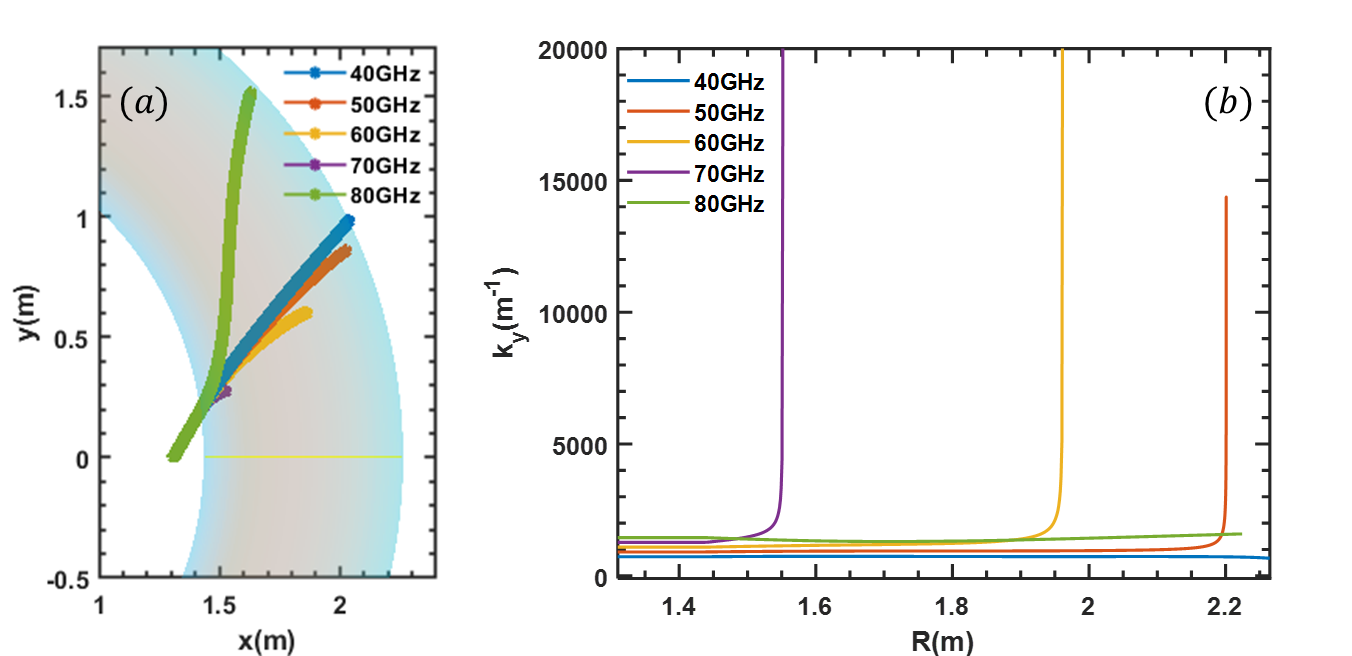
\includegraphics[width=12cm]{image95.png}
\caption{\label{fig:multinout}(a)多个频率X波高场侧注入(b)各频率ky分布图
}
\end{figure}
会穿过1fce共振层,但由于1fce的X模通常光学厚度远小于1,吸收系数低,因此即使在热等离子体中会出现共振吸收,所吸收量也相对微不足道。
对于以上分析可得出如下结论:
\begin{itemize}
\item[(1)]
上杂化频率附近的电磁波具有左旋波特征,最容易实现反常多普勒共振。
\item[(2)]
电子发生快速角度散射时通常伴随着上杂化波产生,通过高场侧注入电磁波激发上杂化波,理论上可以实现对共振区间的逃逸电子能量散射约束。
\item[(3)]
随着托卡马克装置中等离子体密度变化,注入电磁波对应的共振层位置也随之发生改变。由于理论上逃逸电子约束所需电磁波的能量要求最多为KW量级,对仪器的要求较低,可以通过密度诊断时时调节频率参数以实现固定位置的共振散射,例如聚焦在等离子体芯部,逃逸电子容易在等离子体芯部获得稳定的加速环境。
\end{itemize}

\section{小结}
本章首先介绍了非热化电子动理学求解过程,并通过各种标准物理模型验证计算结果的准确性,为下一章实验现象的数值分析提供计算平台。针对反常多普勒共振,本章通过模拟均匀磁场下电子与电磁波的共振发现ADE主要是由具有左旋圆偏振的电磁波产生,当电磁波能量超过一定阈值时,电磁波可以通过ADE实现对共振电子持续的动量散射,验证了模拟和量子对ADE效应描述的一致性。结合托卡马克中本征模分析和射线追迹程序,本章对利用电磁波抑制逃逸电子的方法进行了探讨,并对通过托卡马克高场测注入X波抑制逃逸电子的方法进行了分析。
  \par 本章的动理学程序相对于21世纪出现的经典动理学求解程序的优劣比较如\autoref{table:CompCode}所示。相对于CODE和Norse程序,本文程序主要优势是采用了最完备的雪崩碰撞算符以及新引入了磁扰动算符,通过结合电子回旋辐射模块使得我们的计算结果和实验拥有了直接对比的媒介。

\begin{table*}[h]
  \centering

\caption{\label{table:CompCode}Kinetic 算法与经典计算程序优劣比较}
\begin{tabular}{lccc}
  \hline
 \multirow{2}{*}{} & CODE\cite{RN814}&Norse\cite{RN1894} &Kinetic \\
  & (2014) & (2017)& (2023)\\
  \hline
  背景场分布 & 均匀 & 均匀 & 均匀\\
  \hline
 维度 & 0D2P & 0D2P &0D2P\\
 \hline
 算法 & 谱方法 & 有限差分 &谱方法\\
 \hline
 跨模块兼容性 & 未知 & 强 &强\\
 \hline
电场 & $\checkmark$ & $\checkmark$ &$\checkmark$\\
辐射阻尼& $\times$ & $\checkmark$ &$\checkmark$\\
Fokker-Planck碰撞项&  $\checkmark$ & $\checkmark$ &$\checkmark$\\
雪崩碰撞项& Rosenbluth term\cite{RN1793}(1997)& Chiu term\cite{RN1941}(1998) &O. Embréus term\cite{RN1811}(2018)\\
背景电子演化项& $\times$ &$\checkmark$ &$\times$\\
磁扰动项&$\times$ & $\times$&$\checkmark$\\
\hline
可时变参数输入&未知& $\checkmark$&$\checkmark$\\
\hline
电子回旋辐射模块&$\times$& $\times$&$\checkmark$ \\
\hline
\end{tabular}
\end{table*}


%\begin{table*}[h]
%  \centering
%\begin{sideways}
%\caption{\label{table:CompCode}Kinetic 算法与经典计算程序优劣比较}
%\begin{tabular}{lccc}
%  \hline
% \multirule{2}{*}{} & CODE\cite{RN814}&Norse\cite{RN1894} &Kinetic \\
%  & (2014) & (2017)& (2023)\\
%  \hline
%  背景场分布 & 均匀 & 均匀 & 均匀\\
%  \hline
% 维度 & 0D2P & 0D2P &0D2P\\
% \hline
% 算法 & 谱方法 & 有限差分 &谱方法\\
% \hline
% 跨模块兼容性 & 未知 & 强 &强\\
% \hline
%电场 & $\checkmark$ & $\checkmark$ &$\checkmark$\\
%辐射阻尼& $\times$ & $\checkmark$ &$\checkmark$\\
%Fokker-Planck碰撞项&  $\checkmark$ & $\checkmark$ &$\checkmark$\\
%雪崩碰撞项& Rosenbluth term\cite{RN1793}(1997)& Chiu term\cite{RN1941}(1998) &O. Embréus term\cite{RN1811}(2018)\\
%背景电子演化项& $\times$ &$\checkmark$ &$\times$\\
%磁扰动项&$\times$ & $\times$&$\checkmark$\\
%\hline
%可时变参数输入&未知& $\checkmark$&$\checkmark$\\
%\hline
%电子回旋辐射模块&$\times$& $\times$&$\checkmark$ \\
%\hline
%\end{tabular}
%\end{sideways}
%\end{table*}





